%%%%%%%%%%%%%%%%%%%%%%%%%%%%%
% Standard header for working papers
%
% WPHeader.tex
%
%%%%%%%%%%%%%%%%%%%%%%%%%%%%%

\documentclass[11pt]{article}



%%%%%%%%%%%%%%%%%%%%%%%%%%
%% TEMPLATES
%%%%%%%%%%%%%%%%%%%%%%%%%%


% Simple Tabular

%\begin{tabular}{ |c|c|c| } 
% \hline
% cell1 & cell2 & cell3 \\ 
% cell4 & cell5 & cell6 \\ 
% cell7 & cell8 & cell9 \\ 
% \hline
%\end{tabular}





%%%%%%%%%%%%%%%%%%%%%%%%%%
%% Packages
%%%%%%%%%%%%%%%%%%%%%%%%%%



% encoding 
\usepackage[utf8]{inputenc}
\usepackage[T1]{fontenc}


% general packages without options
\usepackage{amsmath,amssymb,amsthm,bbm}

% graphics
\usepackage{graphicx,transparent,eso-pic}

% text formatting
\usepackage[document]{ragged2e}
\usepackage{pagecolor,color}
%\usepackage{ulem}
\usepackage{soul}


% conditions
\usepackage{ifthen}


\usepackage{natbib}


%%%%%%%%%%%%%%%%%%%%%%%%%%
%% Maths environment
%%%%%%%%%%%%%%%%%%%%%%%%%%

%\newtheorem{theorem}{Theorem}[section]
%\newtheorem{lemma}[theorem]{Lemma}
%\newtheorem{proposition}[theorem]{Proposition}
%\newtheorem{corollary}[theorem]{Corollary}

%\newenvironment{proof}[1][Proof]{\begin{trivlist}
%\item[\hskip \labelsep {\bfseries #1}]}{\end{trivlist}}
%\newenvironment{definition}[1][Definition]{\begin{trivlist}
%\item[\hskip \labelsep {\bfseries #1}]}{\end{trivlist}}
%\newenvironment{example}[1][Example]{\begin{trivlist}
%\item[\hskip \labelsep {\bfseries #1}]}{\end{trivlist}}
%\newenvironment{remark}[1][Remark]{\begin{trivlist}
%\item[\hskip \labelsep {\bfseries #1}]}{\end{trivlist}}

%\newcommand{\qed}{\nobreak \ifvmode \relax \else
%      \ifdim\lastskip<1.5em \hskip-\lastskip
%      \hskip1.5em plus0em minus0.5em \fi \nobreak
%      \vrule height0.75em width0.5em depth0.25em\fi}



%% Commands

\newcommand{\noun}[1]{\textsc{#1}}


%% Math

% Operators
\DeclareMathOperator{\Cov}{Cov}
\DeclareMathOperator{\Var}{Var}
\DeclareMathOperator{\E}{\mathbb{E}}
\DeclareMathOperator{\Proba}{\mathbb{P}}

\newcommand{\Covb}[2]{\ensuremath{\Cov\!\left[#1,#2\right]}}
\newcommand{\Eb}[1]{\ensuremath{\E\!\left[#1\right]}}
\newcommand{\Pb}[1]{\ensuremath{\Proba\!\left[#1\right]}}
\newcommand{\Varb}[1]{\ensuremath{\Var\!\left[#1\right]}}

% norm
\newcommand{\norm}[1]{\left\lVert #1 \right\rVert}



% argmin
\DeclareMathOperator*{\argmin}{\arg\!\min}


% amsthm environments
\newtheorem{definition}{Definition}
\newtheorem{proposition}{Proposition}
\newtheorem{assumption}{Assumption}

%% graphics

% renew graphics command for relative path providment only ?
%\renewcommand{\includegraphics[]{}}


\usepackage{url}





% geometry
\usepackage[margin=2cm]{geometry}



% changes

\usepackage{soul}
\soulregister\cite7
\soulregister\citep7
\soulregister\ref7

\usepackage[final]{changes}
%\usepackage{changes}


\setaddedmarkup{\textcolor{black}{\hl{#1}}}
\setdeletedmarkup{\textcolor{red}{\sout{#1}}}



\usepackage{CJKutf8}
%\begin{CJK*}{UTF8}{zhsong}
%文章内容。
%\clearpage\end{CJK*}
\newcommand{\cn}[1]{
  \begin{CJK*}{UTF8}{gbsn}
  #1
  \end{CJK*}
}



% layout : use fancyhdr package
%\usepackage{fancyhdr}
%\pagestyle{fancy}
%
%\makeatletter
%
%\renewcommand{\headrulewidth}{0.4pt}
%\renewcommand{\footrulewidth}{0.4pt}
%\fancyhead[RO,RE]{}
%\fancyhead[LO,LE]{Models for the co-evolution of cities and networks}
%\fancyfoot[RO,RE] {\thepage}
%\fancyfoot[LO,LE] {}
%\fancyfoot[CO,CE] {}
%
%\makeatother
%

%%%%%%%%%%%%%%%%%%%%%
%% Begin doc
%%%%%%%%%%%%%%%%%%%%%

\begin{document}







\title{Models for the Co-evolution of Cities and Networks}
\author{\noun{Juste Raimbault}$^{1,2}$\\
$^1$ UPS CNRS 3611 ISC-PIF\\
$^2$ UMR CNRS 8504 G{\'e}ographie-cit{\'e}s
}
\date{}

% current adress vs where the work was realized ?

\maketitle

\justify


\textbf{Keywords : }\textit{Urban System; Co-evolution; Transportation Network}

\medskip


%The complexity of interactions between Networks and Territories has been widely acknowledged empirically, in particular through the existence of circular causal relations in their co-development. A relevant framework to understand this phenomenon is to view it as a \emph{co-evolution}, that we use for territorial systems within Pumain's Evolutive Urban Theory that understands urban systems as complex adaptive systems. Considering modeling as a primary source of indirect knowledge on processes and dynamics, we investigate models endogeneizing this co-evolution, in the particular case of cities and transportation networks. We first proceed to an extended systematic review, based on scientific disciplines mapping through citation network and semantic analysis, in order to shed a light on the existing modeling approaches that span in very diverse disciplines, from planning and urban geography to economics and physics, each having different research questions, ontologies and scales. This systematic review, when consolidated with models purpose, application case, scales and ontologies for objects and processes, yields a modelography including for example land-use Transport Interaction Models, Network growth models or Urban Systems models. This first stage lead us to identify two typical scales at which co-evolution models are relevant, with associated paradigms: the mesoscopic scale in an approach of Urban Morphogenesis, and the macroscopic scale in the context of Evolutive Urban Theory.

%The mesoscopic model we develop has a fine resolution (under 1km) and intermediate spatial extent (50$\sim$100km). Given a fixed exogenous growth rate, population are dispatched following a preferential attachment that depends on a potential controlled by local urban form (density, distance to network) and network measures (centralities and generalized accessibilities), and then diffused in space to capture urban sprawl. Network growth is included through a multi-modeling paradigm: implemented heuristics include biological network generation and gravity potential breakdown. The model is calibrated on measures for Urban Form and network topology, computed on windows spanning full European Union and China, given population density data and OpenStreetMap road network. The calibration is static in the sense that fit is done on final configurations only, but is done at the first (measures) and second (correlations) order, the later capturing indirectly relations between the network and the urban frame. The model is able to reproduce most of existing configurations. The study of lagged correlations within synthetic model runs furthermore unveils a large variety of causality regimes, confirming the ability of the model to grasp the complexity of situations existing empirically.

%At the macroscopic scale, growth rates are endogenous and interactions between cities are their main driver. As a deterministic extension of the Gibrat model, our model considers gravity-based flows within the network to determine growth rates. These have an effect at the first order (direct interaction) but also at the second order (effect of cumulated flows on traversed cities) what allows to capture centrality effects. Network growth follows a demand-induced thresholded growth scheme, that can occur at the global level or locally. The exploration of the model on synthetic city systems unveils patterns of complexity compared to a basic interaction model without co-evolution. We apply the model on the French city system, with population data spanning 1831-1999. We compare behaviors with different network data, namely dynamical railway network (1850-2000) and dynamical highway network (1950-2000). Proceeding to locally stationary in time calibrations, we find that cities population prediction are always more accurate than a static model, even when controlling on additional number of parameters with a specifically designed empirical AIC criterion. Concerning accuracy of generated network, the model is more performant with the highway network, probably because of the multiple regimes that existed in railway history.

%These complementary modeling efforts pave the way for future research towards operational models, with applications in local and territorial planning by helping to design policies integrating transportation and urban development in a dynamical and strongly coupled way.






%\begin{abstract}

%\end{abstract}


%%%%%%%%%%%%%%%%%%%%
\section{Introduction}






\subsection{Models of co-evolution}

We can now switch to models that integrate dynamically the paradigm Territory $\leftrightarrow$ Network, which as we recall assumes that the conditioning of one by the other can not be identified. The ontologies used, as we will see, often couple\footnote{We recall the definition of model coupling, which corresponds to the one of system or process coupling given in introduction: it is the construction of a model that is simultaneously the extension of each initial model.} network elements with territorial components, but this positioning is not necessary and some elements may be hybrid (for example a governance structure for the transportation network may simultaneously belong to both aspects). In our reading of models, these different specifications will naturally arise.

We will broadly designate by model of co-evolution simulation models that include a coupling of urban growth dynamics and transportation network growth dynamics. These are relatively rare, and for most of them still at the stage of stylized models. The efforts being relatively sparse and in very different domains, there is not much unity in these approaches, beside the abstraction of the assumption of an interdependency between networks and territorial characteristics in time. We propose to review them still through the prism of scales.

\subsubsection{Microscopic and mesoscopic scales}


\paragraph{Geometrical Models}

\cite{achibet2014model} describes a co-evolution model at a very large scale (scale of the building), in which evolution of both network and buildings are ruled by a same agent, influenced differently by network topology and population density, and that can be understood as an agent of urban development. The model allows to simulate an auto-organized urban extension and to produce district configurations. Even if it strongly couples territorial components (buildings) and the road network, described results do not imply any conclusion on the processes of co-evolution themselves.

A generalization of the geometrical local optimization model described before is developed in~\cite{barthelemy2009co}. It aims at capturing the co-evolution of network topology with the density of its nodes. The localization of new nodes is simultaneously influenced by density and centrality, yielding the looping of the strong coupling. More precisely, the global behavior of the model is the same, as the network extension behavior. Centers then localize following a utility function that is a linear combination of average betweenness centrality in a neighborhood and of the opposite of density (dispersion due to higher price as a function of density). This utility is used to compute the probability of localization of new centers following a discrete choices model. The model allows to show that the influence of centrality reinforces aggregation phenomena (in particular through an analytical resolution on a one-dimensional version of the model), and furthermore reproduces exponentially decreasing density profiles (Clarcke's law) which are observed empirically.  


\cite{ding2017heuristic} introduce a model of co-evolution between different layers of the transportation network, and show the existence of an optimal coupling parameter in terms of inequalities for the centrality in network conception: if the road network is assimilated at a fine granularity to a population distribution, this model can be compared with the precedent model of co-evolution between the transportation network and the territory.




\paragraph{Economic models}



\cite{levinson2007co} take an economic approach, which is richer from the point of view of network development processes implied, similar to a four step model (i.e. including the generation of origin-destination flows and the assignment of traffic in the network) including travel cost and congestion, coupled with a road investment module simulating toll revenues for constructing agents, and a land-use evolution module updating actives and employments through discrete choice modeling. The exploration experiments show that co-evolving network and land uses lead to positive feedbacks reinforcing hierarchies. These are however far from satisfying, since network topology does not evolve as only capacities and flows change within the network, what implies that more complex mechanisms (such as the planning of new infrastructures) on longer time scales are not taken into account. \cite{li2016integrated} have recently extended this model by adding endogenous real estate prices and an optimization heuristic with a genetic algorithm for deciding agents.


From an other point of view, \cite{levinson2005paving} is also presented as a model of co-evolution, but corresponds more to a predictive model based on Markov chains, and thus closer to a statistical analysis than a simulation model based on these processes. \cite{rui2011urban} describe a model in which the coupling between land-use and network topology is done with a weak paradigm, land-use and accessibility having no feedback on network topology, the land-use model being conditioned to the growth of the autonomous network.




\paragraph{Cellular automatons}


A simple hybrid model explored and applied to a stylized planning example of the functionnal distribution of a new district in~\cite{raimbault2014hybrid}, relies on mechanisms of accessibility to urban activities for the growth of settlements with a network adapting to the urban shape. The rules for network growth are too simple to capture more elaborated processes than just a simple systematic connection (such as potential breakdown for example), but the model produces at a large scale a broad range of urban shapes reproducing typical patterns of human settlements. This model is inspired by~\cite{moreno2012automate} for its core mechanisms but yield a much broader generation of forms by taking into account urban functions.


At these relatively large scales, spanning from the urban to the metropolitan scale, mechanisms of population localization influenced by accessibility coupled to mechanisms of network growth optimizing some particular functions seem to be the rule for this kind of models: in the same way, \cite{wu2017city} couple a cellular automaton for population diffusion to a network optimizing local cost that depends on the geometry and on population distribution.


Models answering to more remote questions can furthermore be linked to our problem: for example, in a conceptual way, a certain form of strong coupling is also used in~\cite{bigotte2010integrated} which by an approach of operational research propose a network design algorithm to optimize the accessibility to amenities, taking into account both network hierarchy and the hierarchy of connected centers.


This way, co-evolution models at the microscopic and mesoscopic scales globally have the following structure: (i) processes of localization or relocalization of activities (actives, buildings) influenced by their own distribution and network characteristics; (ii) network evolution, that can be topological or not, answering to very diverse rules: local optimization, fixed rules, planning by deciding agents. This diversity suggests the necessity to take into account the superposition of multiple processes ruling network evolution.


\subsubsection{Urban systems modeling}

At a macroscopic scale, co-evolution can be taken into account in models of urban systems. \cite{baptiste1999interactions} propose to couple an urban growth model based on migrations (introduced by the application of synergetics to systems of cities by~\cite{sanders1992systeme}) with a mechanism of self-reinforcement of capacities for the road network without topological modification. More precisely, the general principles of the model are the following.
\begin{itemize}
\item Attractivity and repulsion indicators allow for each city to determine emigration and immigration rates and to make populations evolve.
\item Network topology is fixed in time, but capacities of links evolve. The rule is an increase in capacity when the flow becomes greater given a fixed parameter threshold during a given number of iterations. Flows are affected with a gravity model of interaction between cities.
\end{itemize}


The last version of this model is presented by~\cite{baptistemodeling}. General conclusions that can be obtained from this work are that this coupling yield a hierarchical configuration\footnote{But we also know that simpler models, only a preferential for example, allow to reproduce this stylized fact. The model must have as an objective to answer to broader questions, such as the fine understanding of co-evolution processes, what is not done here. However, one of its operational objectives is otherwise fulfilled, through the application to France and the study of the impact of a high speed line project, recalling the multiple possible functions of a model (see~\ref{sec:computation}).} and that the addition of the network produces a less hierarchical space, allowing medium-sized cities to benefit from the feedback of the transportation network.


The model proposed by~\cite{blumenfeld2010network} can be seen as a bridge between the mesoscopic scale and the approaches of urban systems, since it simulates migrations between cities and network growth induced by potential breakdown when detours are too large. In the continuity of Simpop models for systems of cities, \cite{schmitt2014modelisation} describes the SimpopNet model which aims at precisely integrating co-evolution processes in systems of cities on long time scales, typically via rules for hierarchical network development as a function of the dynamics of cities, coupled with these that depends on network topology. Unfortunately the model was not explored nor further studied, and furthermore stayed at a toy-level. \cite{cottineau2014evolution} proposes an endogenous transportation network growth as the last building brick of the Marius modeling framework, but it stays at a conceptual level since this brick has not been specified nor implemented yet. To the best of our knowledge, there exists no model which is empirical or applied to a concrete case based on an approach of co-evolution by urban systems from the point of view of the evolutive urban theory.



We can see well the opposition to epistemological principles of economic geography: \cite{fujita1999evolution} introduce for example an evolutionary model able to reproduce and urban hierarchy and an organization typical of central place theory~\cite{banos2011christaller}, but that still relies on the notion of successive equilibriums, and moreover considers a ``Krugman-like'' model, i.e. a one dimensional and isotropic space, in which agents are homogeneously distributed\footnote{The absence of a real space is not an issue in this economic approach that aims at understanding processes out of their context. In our case, the structure of the geographical space is not separable, and indeed at the core of the issues we are interested in.}. This approach can be instructive on economic processes in themselves but more difficultly on geographical processes, since these imply the embedding of economic processes in the geographical space which spatial particularities not taken into account in this approach are crucial. Our work will focus on demonstrating to what extent this structure of space can be important and also explicative, since networks, and even more physical networks induce spatio-temporal processes that are path-dependent and thus sensitive to local singularities and prone to bifurcations induced by the combination of these with processes at other scales (for example the centrality inducing a flow).


At the macroscopic scale, existing models are based on the evolution of agents (generally cities) as a consequence of their interactions, carried by the network, whereas the evolution of the network can follow different rules: self-reinforcement, potential breakdown. The general structure is globally the same than at larger scales, but ontologies stay fundamentally different.





%%%%%%%%%%%%%%%%%%%%
\section{Specification of co-evolution models}

This section extends the logic of integrating a system of cities with a transportation network, which has been pursued in a static way for network behavior in the interaction model developed and explored in section~\ref{sec:interactiongibrat}, to propose a \emph{macroscopic model of co-evolution for systems of cities}.


\subsection{Rationale}

This first approach relies in a direct extension of the interaction model within a system of cities described in chapter~\ref{ch:evolutiveurban}, at a macroscopic scale with an ontology typical to systems of cities. For the sake of simplicity, we still stick to an unidimensional description of cities by their population.


Concerning network growth, we propose also to stay at a relatively aggregated and simplified level, allowing to test growth heuristics at different levels of abstraction. In order to be flexible on model mechanisms, diverse processes can be taken into account, such as direct interactions between cities, intermediate interactions through the network, the feedback of network flows and a demand-induced network growth.


Empirical characteristics emphasized by~\cite{thevenin2013mapping} for the French railway network suggest the existence of feedbacks of network use, or of flows traversing it, on its persistence and its development, whose properties have evolved in time: a first phase of strong development would correspond to an answer to a high need of coverage, followed by a reinforcement of main link and the disappearance of weakest links.


The coupling between cities and the network will be achieved by the intermediate of flows between cities in the network: these capture the interactions between cities and have simultaneously an influence on the network in which they flow.


%%%%%%%%%%%%%%%%%
\begin{figure}
\includegraphics[width=\linewidth]{figures/model}
\caption[Schematic model representation]{\textbf{Abstract representation of the model.} Ellipses correspond to main ontological elements (cities, network, flows), whereas arrows translate processes for which associated parameters are given. The model is described in its broader ecosystem of initialisation and output indicators.\label{fig:macrocoevol:model}}
\end{figure}
%%%%%%%%%%%%%%%%%


\subsection{Model description}

The urban system is characterized by populations $\mu_i(t)$ and the network $\mathbf{G}(t)$, to which can be associated a distance matrix $d^G_{ij}(t)$. Flows between cities $\phi_{ij}$ follow the expression given in~\ref{sec:interactiongibrat} with network distance. The same way, the evolution of populations follows the specifications of the base model. The Fig.~\ref{fig:macrocoevol:model} shows the structure of the model.


Concerning the network, we assume that it evolves following the equation
\begin{equation}
\mathbf{G}(t + 1) = F(\mathbf{G}(t),\phi_{ij}(t))
\end{equation}
such that the assignment of flows within the network and a local variation of its elements is possible. We propose in a first time to consider patterns linked to distance only, and to specify a relation on an abstract network as
\begin{equation}
d^G_{ij}(t+1) = F(d^G_{ij}(t),\phi_{ij}(t))
\end{equation}
i.e. an evolution of the distance matrix only. In this spirit, we keep an interaction model strictly at a macroscopic scale, since a precise spatialization of the network would imply to take into account a finer scale that includes the local shape of the network which determines shortest paths.



Following a thresholded feedback heuristic, given a flow $\phi$ in a link, we assume its effective distance to be updated by:

\begin{equation}
d(t+1) = d(t)\cdot \left( 1 + g_{max} \cdot \left[\frac{1 - \left(\frac{\phi}{\phi_0}\right)^{\gamma_s}}{1 + \left(\frac{\phi}{\phi_0}\right)^{\gamma_s}}\right]\right)
\end{equation}

with $\gamma_s$ a hierarchy parameter, $\phi_0$ the threshold parameter and $g_{max}$ the maximal growth rate at each step. This auto-reinforcement function can be interpreted the following way: above a limit flow $\phi_0$, the travel conditions improve, whereas they deteriorate below. The hierarchy of gain is given by $\gamma_s$, and since $\frac{1 - \left(\frac{\phi}{\phi_0}\right)^{\gamma_s}}{1 + \left(\frac{\phi}{\phi_0}\right)^{\gamma_s}} \rightarrow_{\phi\rightarrow \infty} -1$, $g_{max}$ is the maximal distance gain. This function is similar to the one used by \cite{tero2007mathematical}\footnote{Which uses $\Delta d = \Delta t \left[ \frac{\phi^\gamma}{1 + \phi^\gamma} - d\right]$. This function yield similarly a threshold effect, since the derivative vanishes at $\phi^{\ast} = \left(\frac{d}{1 - d}\right)^{1/\gamma}$, but it can not be adjusted.}.



\subsection{Indicators}



%


%%%%%%%%%%%%%%%%%%%%
\section{Results}


\subsection{Implementation}

The coupling of the interaction model to a finer representation of the network (for example an encoding of the whole network structure) makes the full integration into an OpenMole plugin more difficult, as it was done for the model studied in~\ref{sec:interactiongibrat}. We need here an \emph{ad hoc} implementation. The use of a workflow as a mediator for coupling is an interesting solution but which is realistic only for a weak coupling as in~\ref{sec:correlatedsyntheticdata}. One of the issues that the meta-modeling library for OpenMole that is currently being developed around OpenMole will have to tackle is the possibility to allow strong coupling (for example in the sense of a dynamical coupling during the evolution of the simulation) of heterogeneous components in a transparent way, in order to benefit from the advantages of different languages or of already existing implementations. 

We choose here a full implementation with NetLogo, for the simplicity of coupling between components. A particular care is taken for the duality of network representation, both as a distance matrix and as a physical network, in order to facilitate the extension to physical network heuristics.



\subsection{Exploration on a synthetic system of cities}


The model is first tested and explored on synthetic city systems, in order to understand some of its intrinsic properties. In this case, we consider the model with an abstract network as specified above, i.e. without spatial description of the network and with evolution rules acting directly on $d^G_{ij}$ given the previous specifications. 


A synthetic city system is generated following the heuristic used in the previous section: (i) $N_S$ cities are randomly distributed in the euclidian plan; (ii) populations are attributed to cities following an inverse power law, with a hierarchy parameter $\alpha_S$ and such that the largest city has a population equal to $P_{max}$, i.e. following $P_i = P_{max} \cdot i^{-\alpha_S}$.


To simplify, several meta-parameters are fixed: the number of cities is fixed at $N_S = 30$, the maximal population at $P_{max} = 100000$ and the maximal network growth to $g_{max} = 0.005$. Final time is fixed at $t_f = 30$, what corresponds to distances divided approximatively by 5\footnote{Indeed, we can compute that the minimal multiplicative factor for distance is $(1 - g_{max})^{t_f}$, what gives for these values $(1 - 0.05)^{30} \simeq 0.214$, i.e. a division by 5 of the travel time.}, in order to comply to an empirical constraint: this corresponds to the evolution of the travel time between Paris and Lyon from around ten hours at the beginning of the century to two hours today, showed for example by~\cite{thevenin2013mapping}. We also neglect network effects at the second order by taking $w_N = 0$.


We explore a grid in the parameter space $\alpha_S$, $\phi_0$, $\gamma_s$, $w_G$, $d_G$, $\gamma_G$. We use the indicators introduced in~\ref{sec:macrocoevolexplo} to quantify model behavior in the parameter space. We describe the results for $\alpha_S = 1$, what is the closest to existing city systems (in comparison to 0.5 and 1.5, see the systematic review of the rank-size law estimations done by~\cite{10.1371/journal.pone.0183919}).



L'évolution de la centralité de proximité moyenne dans le temps est visualisée en Fig.~\ref{fig:macrocoevol:behavior-time} (haut) pour $w_G = 0.001$, et à $(\gamma_G,\phi_0)$ variables. Le comportement n'est pas sensible à $d_G$ (voir graphique complet en~\ref{app:sec:macrocoevol}). Cette évolution témoigne d'une transition en fonction du niveau de hiérarchie : lorsque celui-ci décroit, on observe l'émergence de trajectoires où la centralité moyenne croît dans le temps, ce qui correspond à des situations où l'ensemble des villes bénéficie en moyenne d'accroissements d'accessibilité.


Concerning the entropy of populations, for which the temporal trajectory is shown in Fig.~\ref{fig:macrocoevol:behavior-time} (bottom), all parameters give a decreasing entropy, i.e. a behavior of convergence of cities trajectories in time\footnote{Indeed, the entropy for the population variable gives the dispersion of the distribution of populations, and thus its decrease translate a trend to concentrate in time.}.


Looking at the complexity of accessibility trajectories, we observe for values of $\phi_0 > 1.5$ a maximum of complexity as a function of interaction distance $d_G$, stable when $w_G$ and $\gamma_G$ vary (see also the exhaustive plots in Fig.~\ref{fig:app:macrocoevol:behavior-aggreg}, Appendix~\ref{app:sec:macrocoevol}). This intermediate scale can be interpreted as producing regional subsystems, large enough for each to develop a certain level of complexity, et isolated enough to avoid the convergence of trajectories over the whole system. We reconstruct therein a spatial non-stationarity, typically observed in~\ref{sec:staticcorrelations}, and rejoin the concept of the ecological niche\footnote{As it was already described in~\ref{sec:interdiscmorphogenesis}, an ecological niche in the sense of~\cite{holland2012signals} corresponds to the relatively independent ecosystem in which there is co-evolution between the species.} localized in space: the emergent subsystems that are relatively independent, are good candidates to contain processes of co-evolution. The emergence of this intermediate scale can be compared to the modularity of the French urban system showed by~\cite{berroir2017systemes}.



Finally, the behavior of rank correlations for accessibility reveals that the interaction distance systematically increases the number of hierarchy inversions, what corresponds in a sense to an increase in overall system complexity. The hierarchy parameter diminishes this correlation, what means that a more hierarchical organization will impact a larger number of cities in the qualitative aspects of their trajectories. This effect is similar to the ``first mover advantage'' showed by \cite{levinson2011does}, which unveils a path dependency and an advantage to be rapidly connected to the network: in our case, the modifications in the hierarchy correspond to cities that benefit from their positioning in the network.



\subsection{Application to the French system of cities}


The model is then applied to the French system of cities on long time dynamical data: the Pumain-INED database for populations, spanning from 1831 to 1999 \cite{pumain1986fichier}, with the evolving railway network from 1840 to 2000 \cite{thevenin2013mapping}. Such a time span can be associated with structural effect on long time, as developed in~\ref{sec:networkterritories}. This application aims on the one hand at testing the ability of the model to reproduce a real dynamic of co-evolution, and on the other hand at extracting thematic information on processes through calibrated parameter values.

\subsubsection{Data}

We work on railway network data constructed by~\cite{thevenin2013mapping}. The French railway network is particularly interesting jointly with population data already presented, since the covered time span is relatively close, and as \cite{thevenin2013mapping} recalls, this transportation mode has at any times materialized the implication of public and private actors. It corresponds to different processes depending on the period, from a more decentralized management to a more centralized recently, and different technological materializations with for example the recent emergence of high speed trains \cite{zembri1997fondements}. For each date in the population database, we extract the simplified abstract network in which all stations and intersections with a degree larger than two are linked with abstract links which speed and length attributes correspond to real values, at a granularity of 1km\footnote{This processing is achieved thanks to the R package for transportation network analysis specifically developed for this thesis, see~\ref{app:sec:packages}.}. This yields the time-distance matrices between the cities included in the model.



\subsubsection{Stylized facts}


Before calibrating the model, we can observe the lagged correlation patterns in the dataset, by applying the causality regimes method. This empirical study should on the one hand allow us to verify well known stylized facts, and on the other hand to produce a preliminary knowledge of empirical system behavior. We compute as detailed above the closeness centrality through the network, given by $T_i = \sum_j \exp{-d_{ij}/d_0}$, and we study the lagged correlation between its derivative $\Delta T_i$ and the derivative of the population $\Delta P_i$, given by $\hat{\rho}_{\tau} = \hat{\rho}\left[\Delta P_i(t),\Delta T_i(t-\tau)\right]$ estimated on a moving window containing $T_w$ successive dates. We show in Fig.~\ref{fig:macrocoevol:empirical} the results obtained.


These results are important for at least two reasons. First, the behavior of the number of significant correlations as a function of $T_w$ and $d_0$ allows us to find stationarity scales in the system. We observe on the one hand a specific spatial scale that gives a maximum for all temporal windows, at $d_0 = 100km$, what suggests the existence of consistent regional subsystems, which existence is stable in time: indeed, this value corresponds to the interaction distance. It remarkably coincides with the intermediate scale isolated in the synthetic model. On the other hand, long spatial ranges induce an optimal temporal scale, for $T_w = 4$ what corresponds to around twenty years: we identify it as the overall temporal stationarity scale of the system and study the lagged correlations for this value.



Secondly, the behavior of lagged correlations does not seem to comply to the existing literature. At the intermediate spatial scale, the values of $\rho_+,\rho_-$ exhibit no regularity. On the whole system, there is until 1946 close to no significant effect, then no causality between 1946 and 1975 (maximum at $\tau = 0$, non-significant minimum), and a 5 years shift of accessibility causing population after 1968 (the effect staying however doubtful). We do not reproduce the correlation effect between network centrality and place in the urban hierarchy advocated by~\cite{bretagnolle2003vitesse}\footnote{As~\cite{lemoy2017scaling} is not able to reproduce, for density profiles as a function of the distance to the center of European metropolis, the transition that allows~\cite{guerois2008built} to define the peri-urban. These more or less recent works are not reproducible, producing neither code nor data, and giving only a superficial description of the methods, and it is thus impossible to know the origin of the qualitative divergence obtained. A good reproducibility together with the construction of systematic comparisons (\emph{benchmarks}) of models, empirical analysis, that are recent but also to validate old studies, seems to be a reasonable solution to this kind of issue.}, what lead us to question the existence of the ``structural co-evolution'' on long time described by \noun{Bretagnolle} in~\cite{espacegeo2014effets}. What \cite{bretagnolle2003vitesse} obtains is a simultaneous correspondence between growth rate and level of connectivity to the network (and not with network dynamic), but not in our sense a co-evolution, since no statistical relation is furthermore exhibited.



We rejoin the recent results of~\cite{mimeur:hal-01616746} that show the statistical non-significance of the correlation between growth rate and evolution of network coverage and accessibility, at a zero delay. Our results are less precise on the class of cities studied (they differentiate large and small cities, and work on a larger panel), but more general as they study variable delays and accessibility ranges, and are thus complementary.


%%%%%%%%%%%%%
\begin{figure}
	%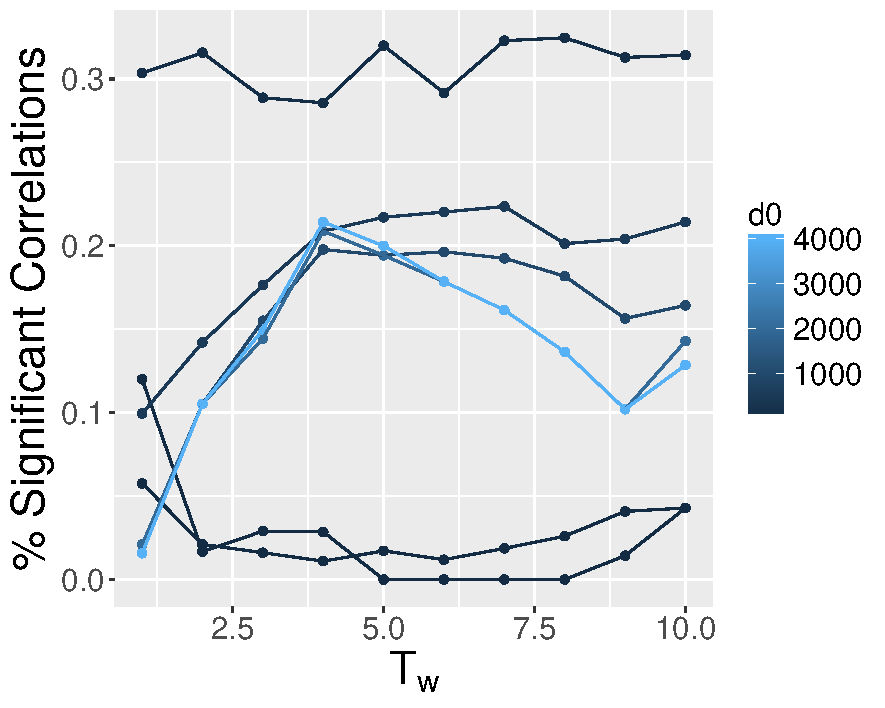
\includegraphics[width=0.48\linewidth]{Figures/MacroCoEvol/significantcorrs_Tw.pdf}
	%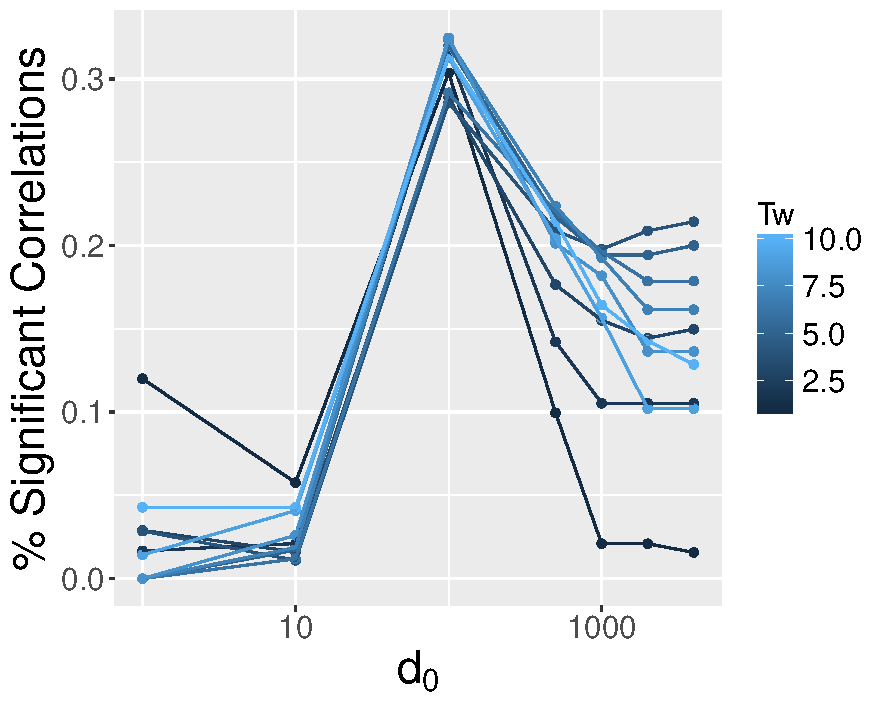
\includegraphics[width=0.48\linewidth]{Figures/MacroCoEvol/significantcorrs_d0.pdf}\\
	%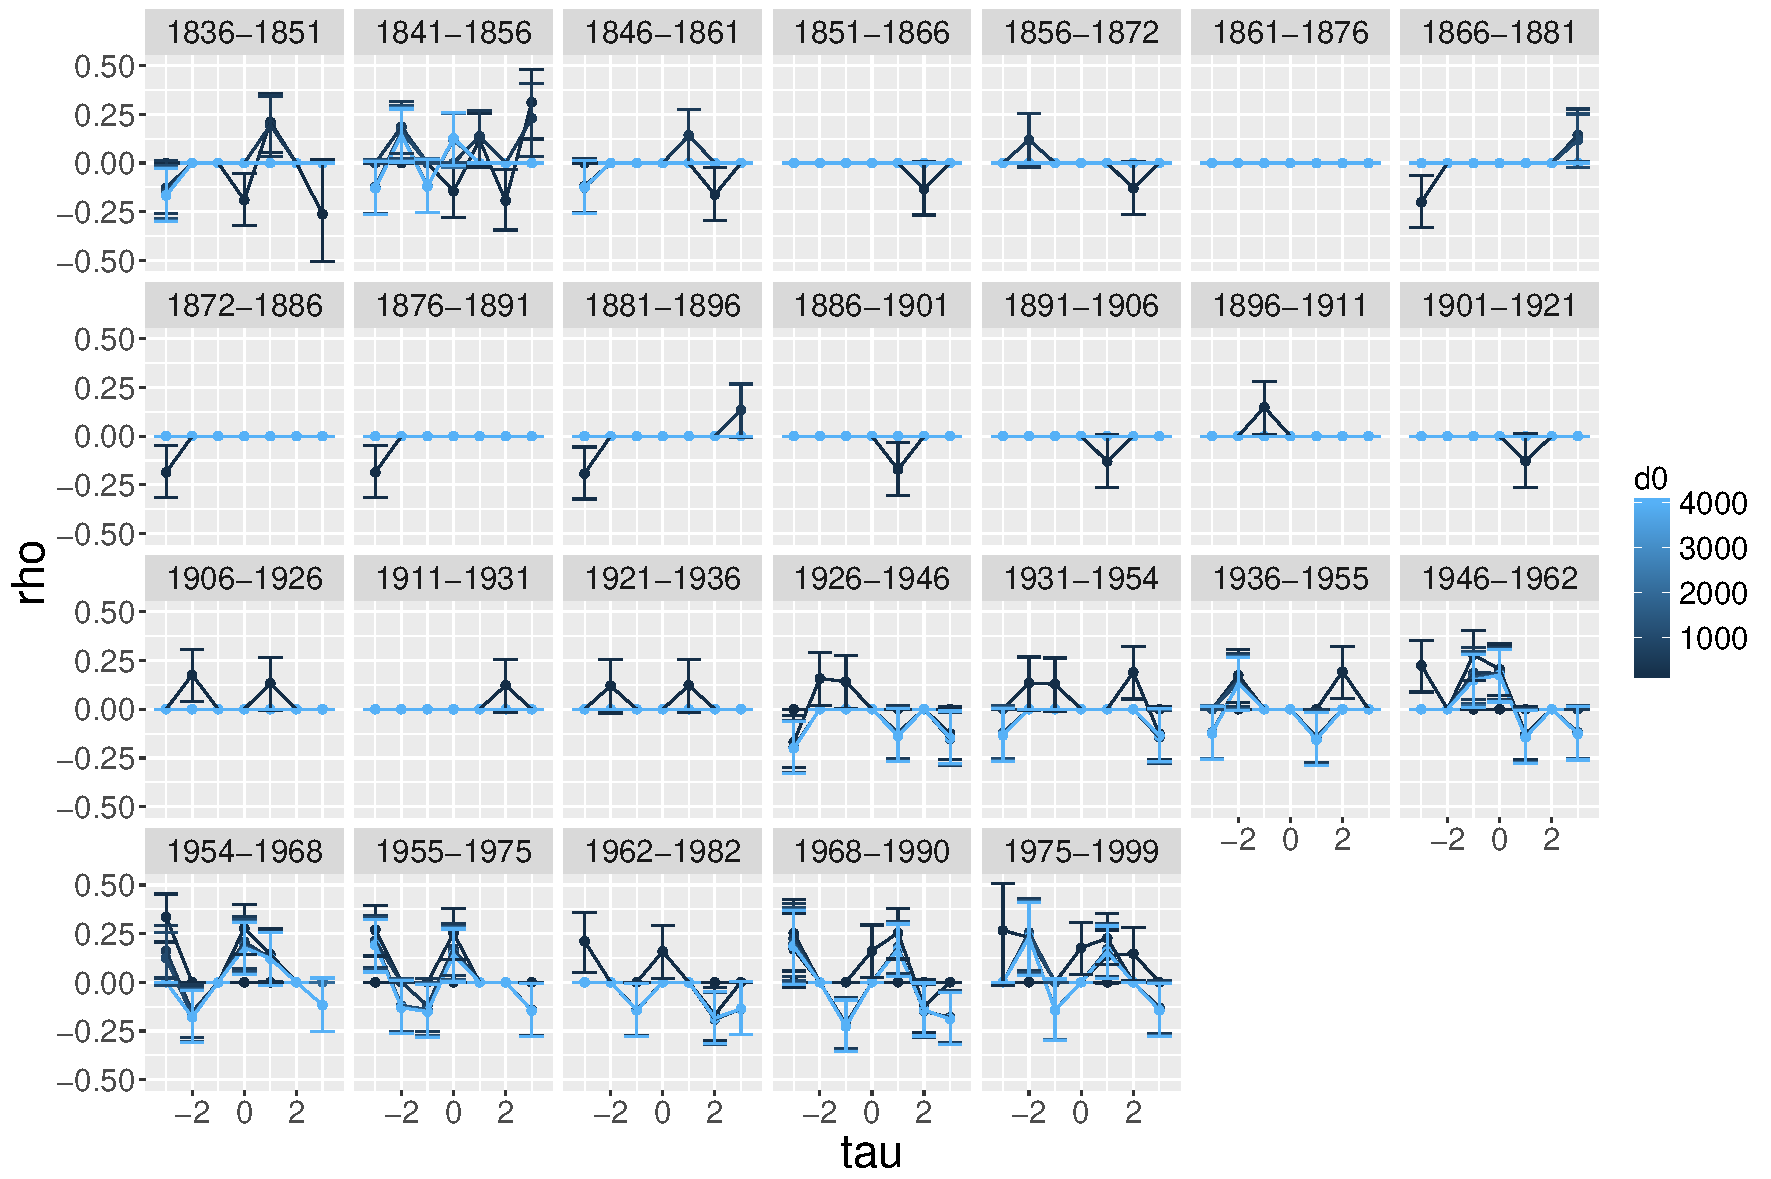
\includegraphics[width=\linewidth]{Figures/MacroCoEvol/laggedCorrs_time_Tw4.pdf}
	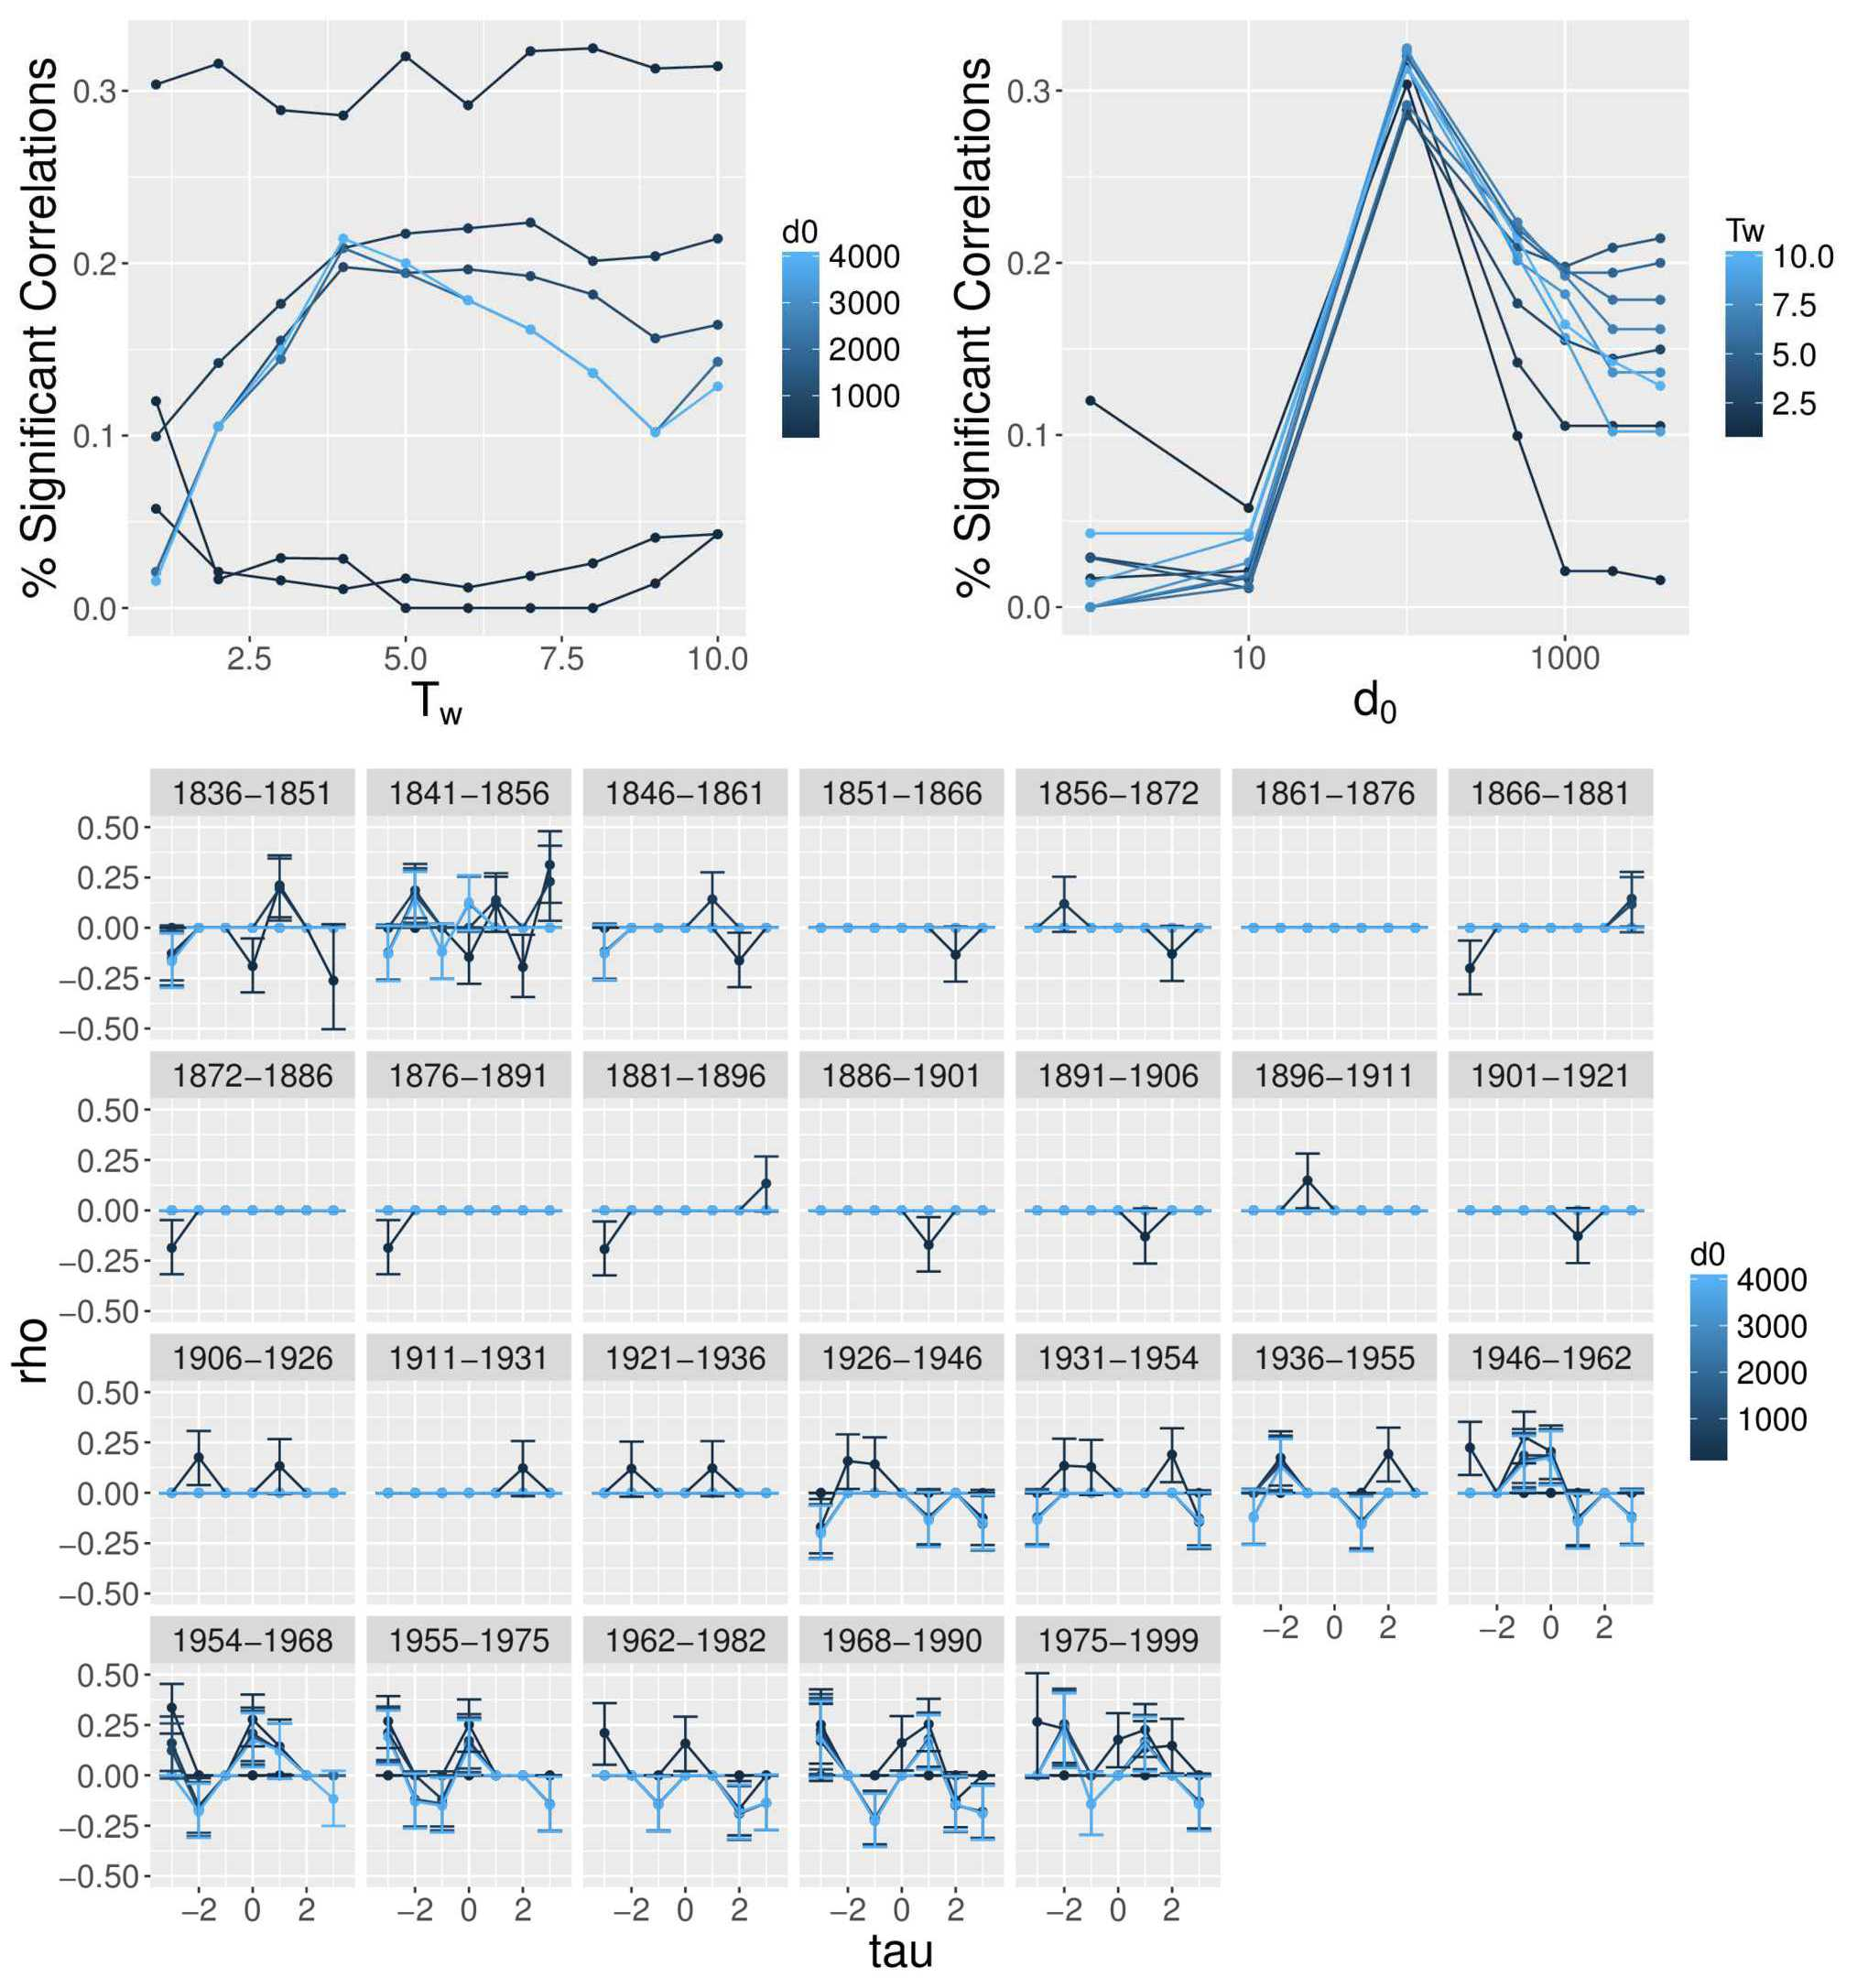
\includegraphics[width=\linewidth]{figures/6-2-3-fig-macrocoevol-empirical.jpg}
	\caption[Empirical lagged correlations for the French system of cities]{\textbf{Empirical lagged correlations for the French system of cities.} Correlations are estimated on a window of duration $5\cdot T_w$, between population growth rates and the variations of closeness centrality with a decay parameter $d_0$ (see text). \textit{(Top left)} Number of significant correlations (taken such that $p<0.1$ at 95\%) as a function of $T_w$ for $d_0$ variable; \textit{(Top right)} Number of significant correlations as a function of $d_0$ for $T_w$ variable; \textit{(Bottom)} For the ``optimal'' window $T_w = 4$, value of $\rho_{\tau}$ as a function of $\tau$, for all successive periods.\label{fig:macrocoevol:empirical}}
\end{figure}
%%%%%%%%%%%%%


\subsubsection{Calibration of the abstract model}


Expected results of the calibration on real data concern both the more or less accurate reproduction of real city population growth dynamics, i.e. to what extent the inclusion of a dynamical network can increase the explanatory power for trajectories, and also how realistic the evolution of network distance is. We still work with the abstract model.


\paragraph{Model evaluation}


We can add to the indicators used before a calibration indicator for distance. The particular property of adjustment for populations, that resides in the existence of a power law for the sizes of cities that made negligible the performance on medium and small cities in the case of a cumulated error, and suggested the addition of the indicator on the error on logarithms, is not present for distances that follow a distribution concentrated on a single order of magnitude. We use therefore a standard measure of fit, given by
\[
\varepsilon_D = \log \left[ \sum_t \sum_{i,j} \left(d_{ij}(t) - \tilde{d}_{ij}(t)\right)^2\right]
\]
where $d_{ij}(t)$ are observed distances and $\tilde{d}_{ij}(t)$ the simulated distances. It is simply a cumulated squared-error, as used for the comparison of origin-destination matrices in a similar case of simulation of a transportation network in~\cite{jacobs2016transport}.


\paragraph{Results}

We proceed to a non-stationary calibration, on the $(\varepsilon_P,\varepsilon_D)$ objectives, i.e. the squared-error on populations and on distances. The estimation is done with a moving window with the periods already used in~\ref{sec:interactiongibrat}. In order to have a limited dimension to explore, we take a fixed $w_N = 0$ to study the interactions only at the first order, knowing that the abstract network parameters $(g_{max},\gamma_S,\varphi_0)$ are taken into account in the calibration. The calibration is done with a genetic algorithm in a way similar as in~\ref{sec:interactiongibrat}. The Fig.~\ref{fig:macrocoevol:pareto} shows the obtained Pareto fronts, and the Fig.~\ref{fig:macrocoevol:parameters} the evolution in time of parameter values for the optimal solutions.

We observe a large variability of the shape of Pareto fronts for the bi-objective calibration on population and distance, what witnesses more or less difficulty to simultaneously adjust population and distance. Some periods, such as 1891-1911 and 1921-1936, are close to have a simultaneous objective point for the two objectives, what would correspond to a good correspondence of the model to both trajectories of cities and trajectory of the network on these periods. 

In comparison with calibration results of the model with static network of~\ref{sec:interactiongibrat}, when comparing the performances for the objective $\varepsilon_G$, we find periods where the static is clearly better (1831 and 1841 for example) and others where the co-evolutive model is better (1946 and 1962): thus, taking into account the co-evolution helps in some cases to have a better reproduction of population trajectories.


The values of optimal parameters in time, shown in Fig.~\ref{fig:macrocoevol:parameters}, seem to contain some signal. The evolution of $w_G$ and $\gamma_G$ are coherent with the evolutions observed for the static model. For $d_G$, the model principally saturates on the maximal distance and the evolution is difficult to interpret. 

However, the evolution of $\phi_0$ could be a sign of a ``TGV effect'' in recent periods, through the secondary peak for population after 1960. Indeed, the construction of high speed lines has shortened distances between cities on top of the hierarchy, and an increase of the threshold $\phi_0$ corresponds to an increase of the selectivity for a potential diminution of distances.


The calibrated $g_{max}$ can finally be interpreted according to the history of the railway network (at least of all points in the Pareto front): a significant secondary peak in the first years, a minimum in the years corresponding to the stabilization of the network (1900), and an increase until today linked to the increase of train speeds and the opening of high speed lines. 


We have this way in a certain extent indirectly quantify interaction processes through the network and the processes of network adaptation to flows, in the case of a real system.


%%%%%%%%%%%%%%%%%%%
\begin{figure}
%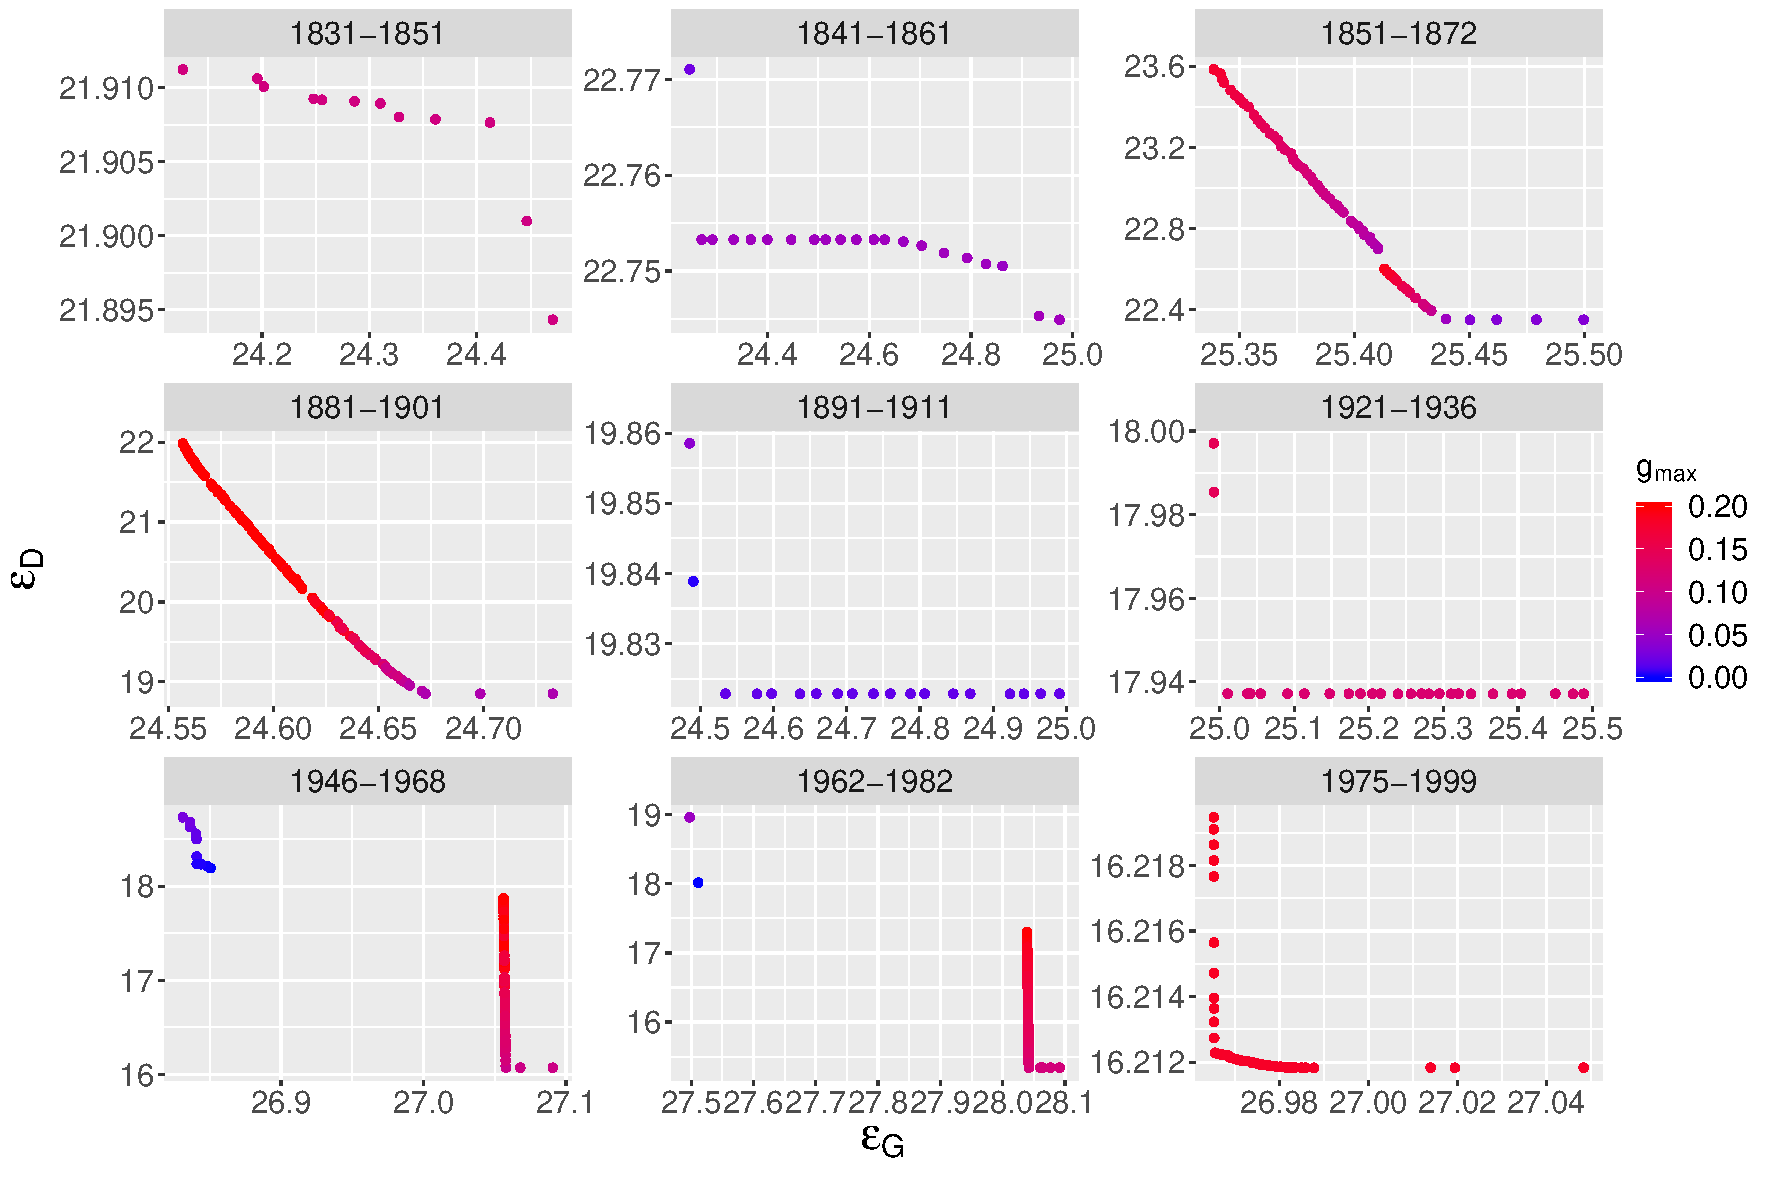
\includegraphics[width=0.9\linewidth]{Figures/MacroCoEvol/pareto_nwGmax_filtTRUE.pdf}
	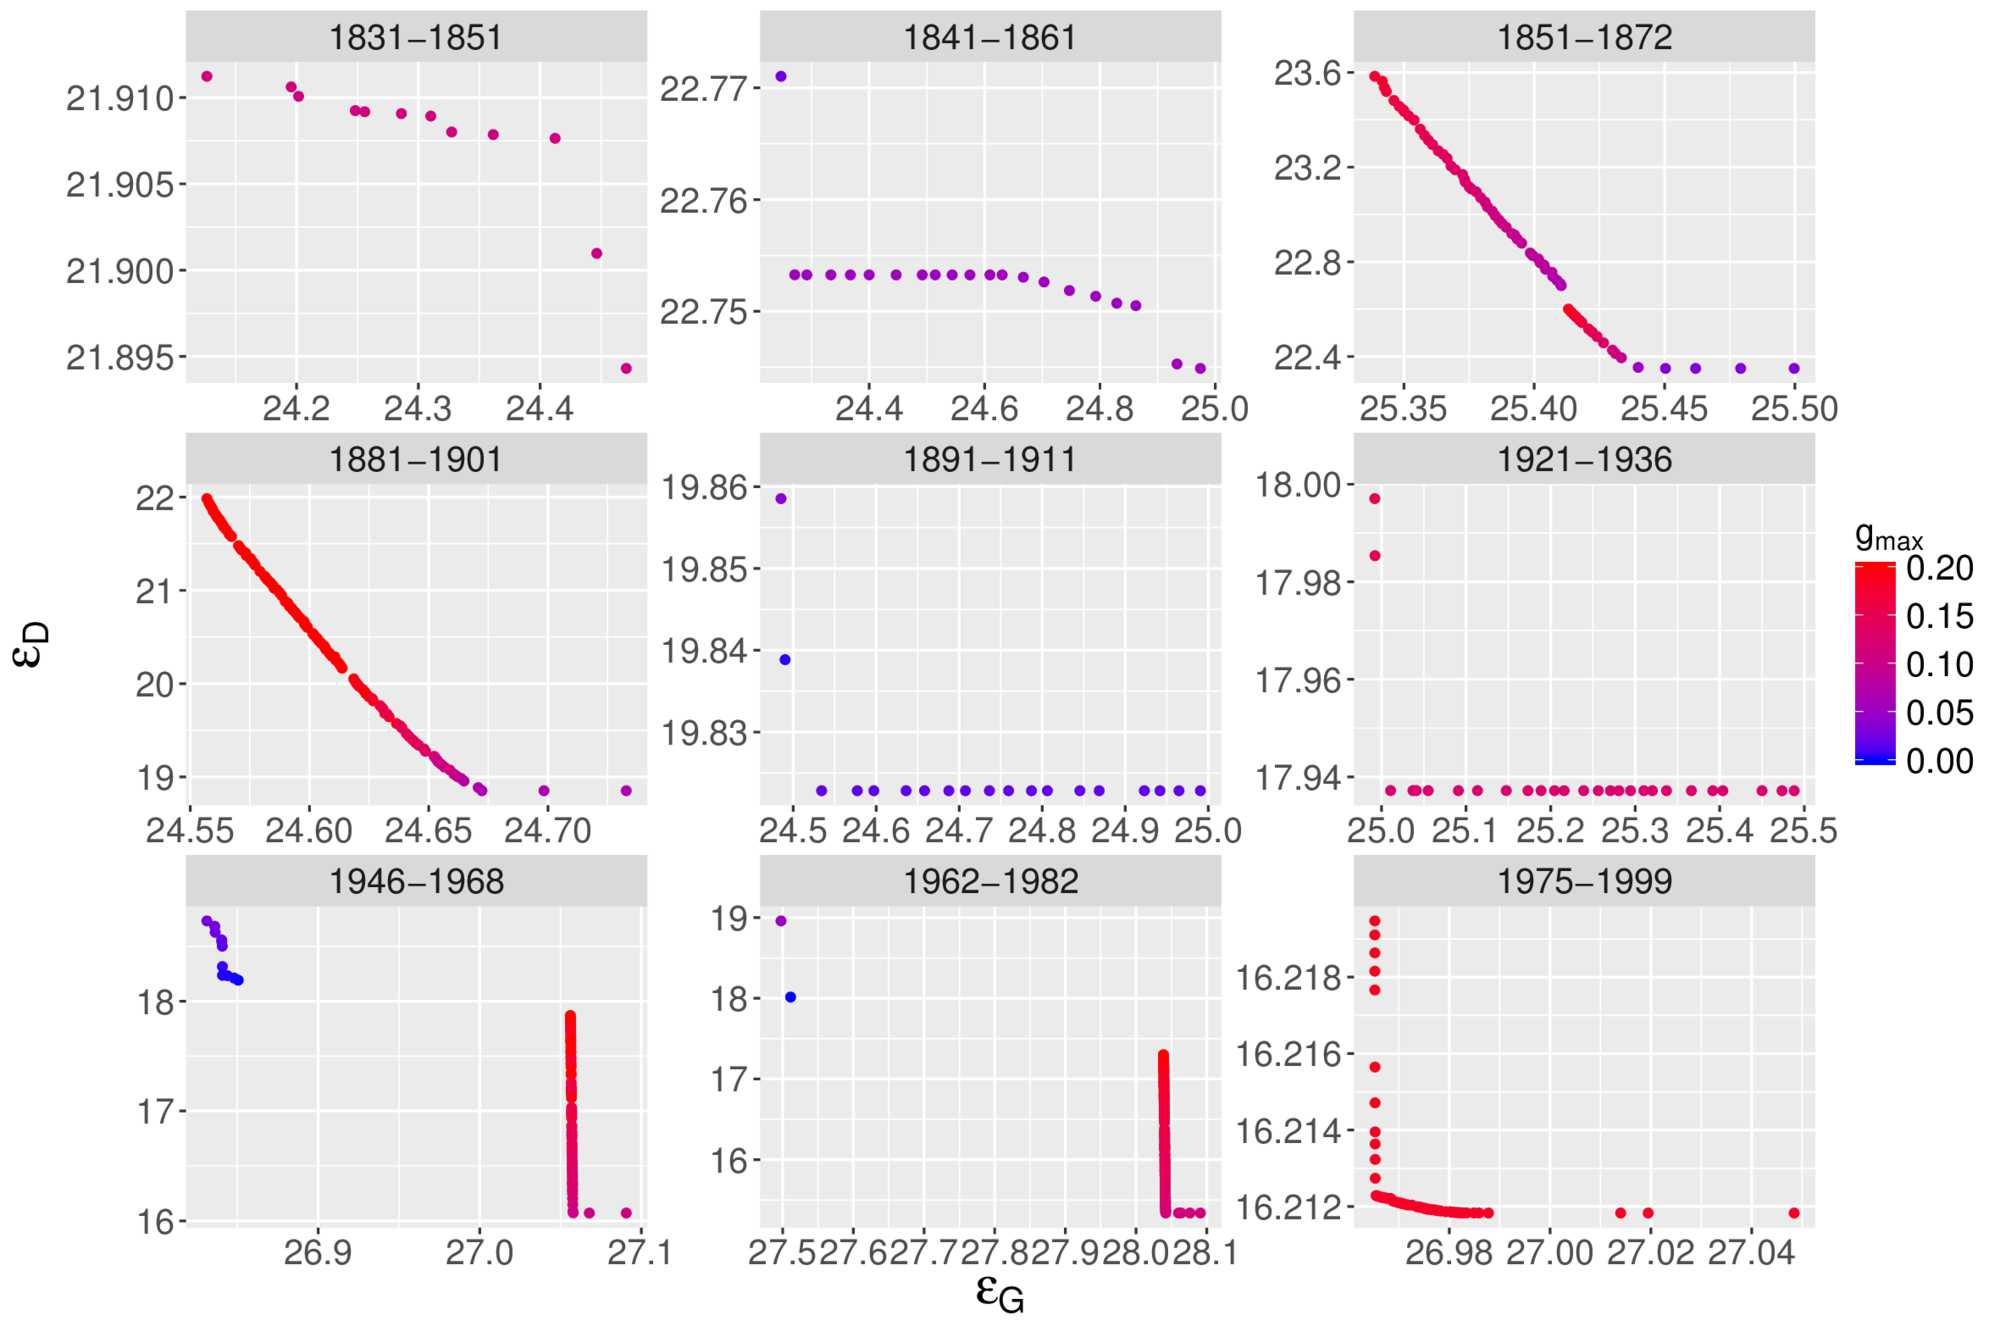
\includegraphics[width=\linewidth]{figures/6-2-3-fig-macrocoevol-pareto.jpg}
	\caption[Pareto fronts for the calibration on population and distance]{\textbf{Pareto fronts for the bi-objective calibration between population and distance.} Fronts are given for each calibration period and are colored according to $g_{max}$.\label{fig:macrocoevol:pareto}}
\end{figure}
%%%%%%%%%%%%%%%%%%%




%%%%%%%%%%%%%%%%%%%
\begin{figure}
	%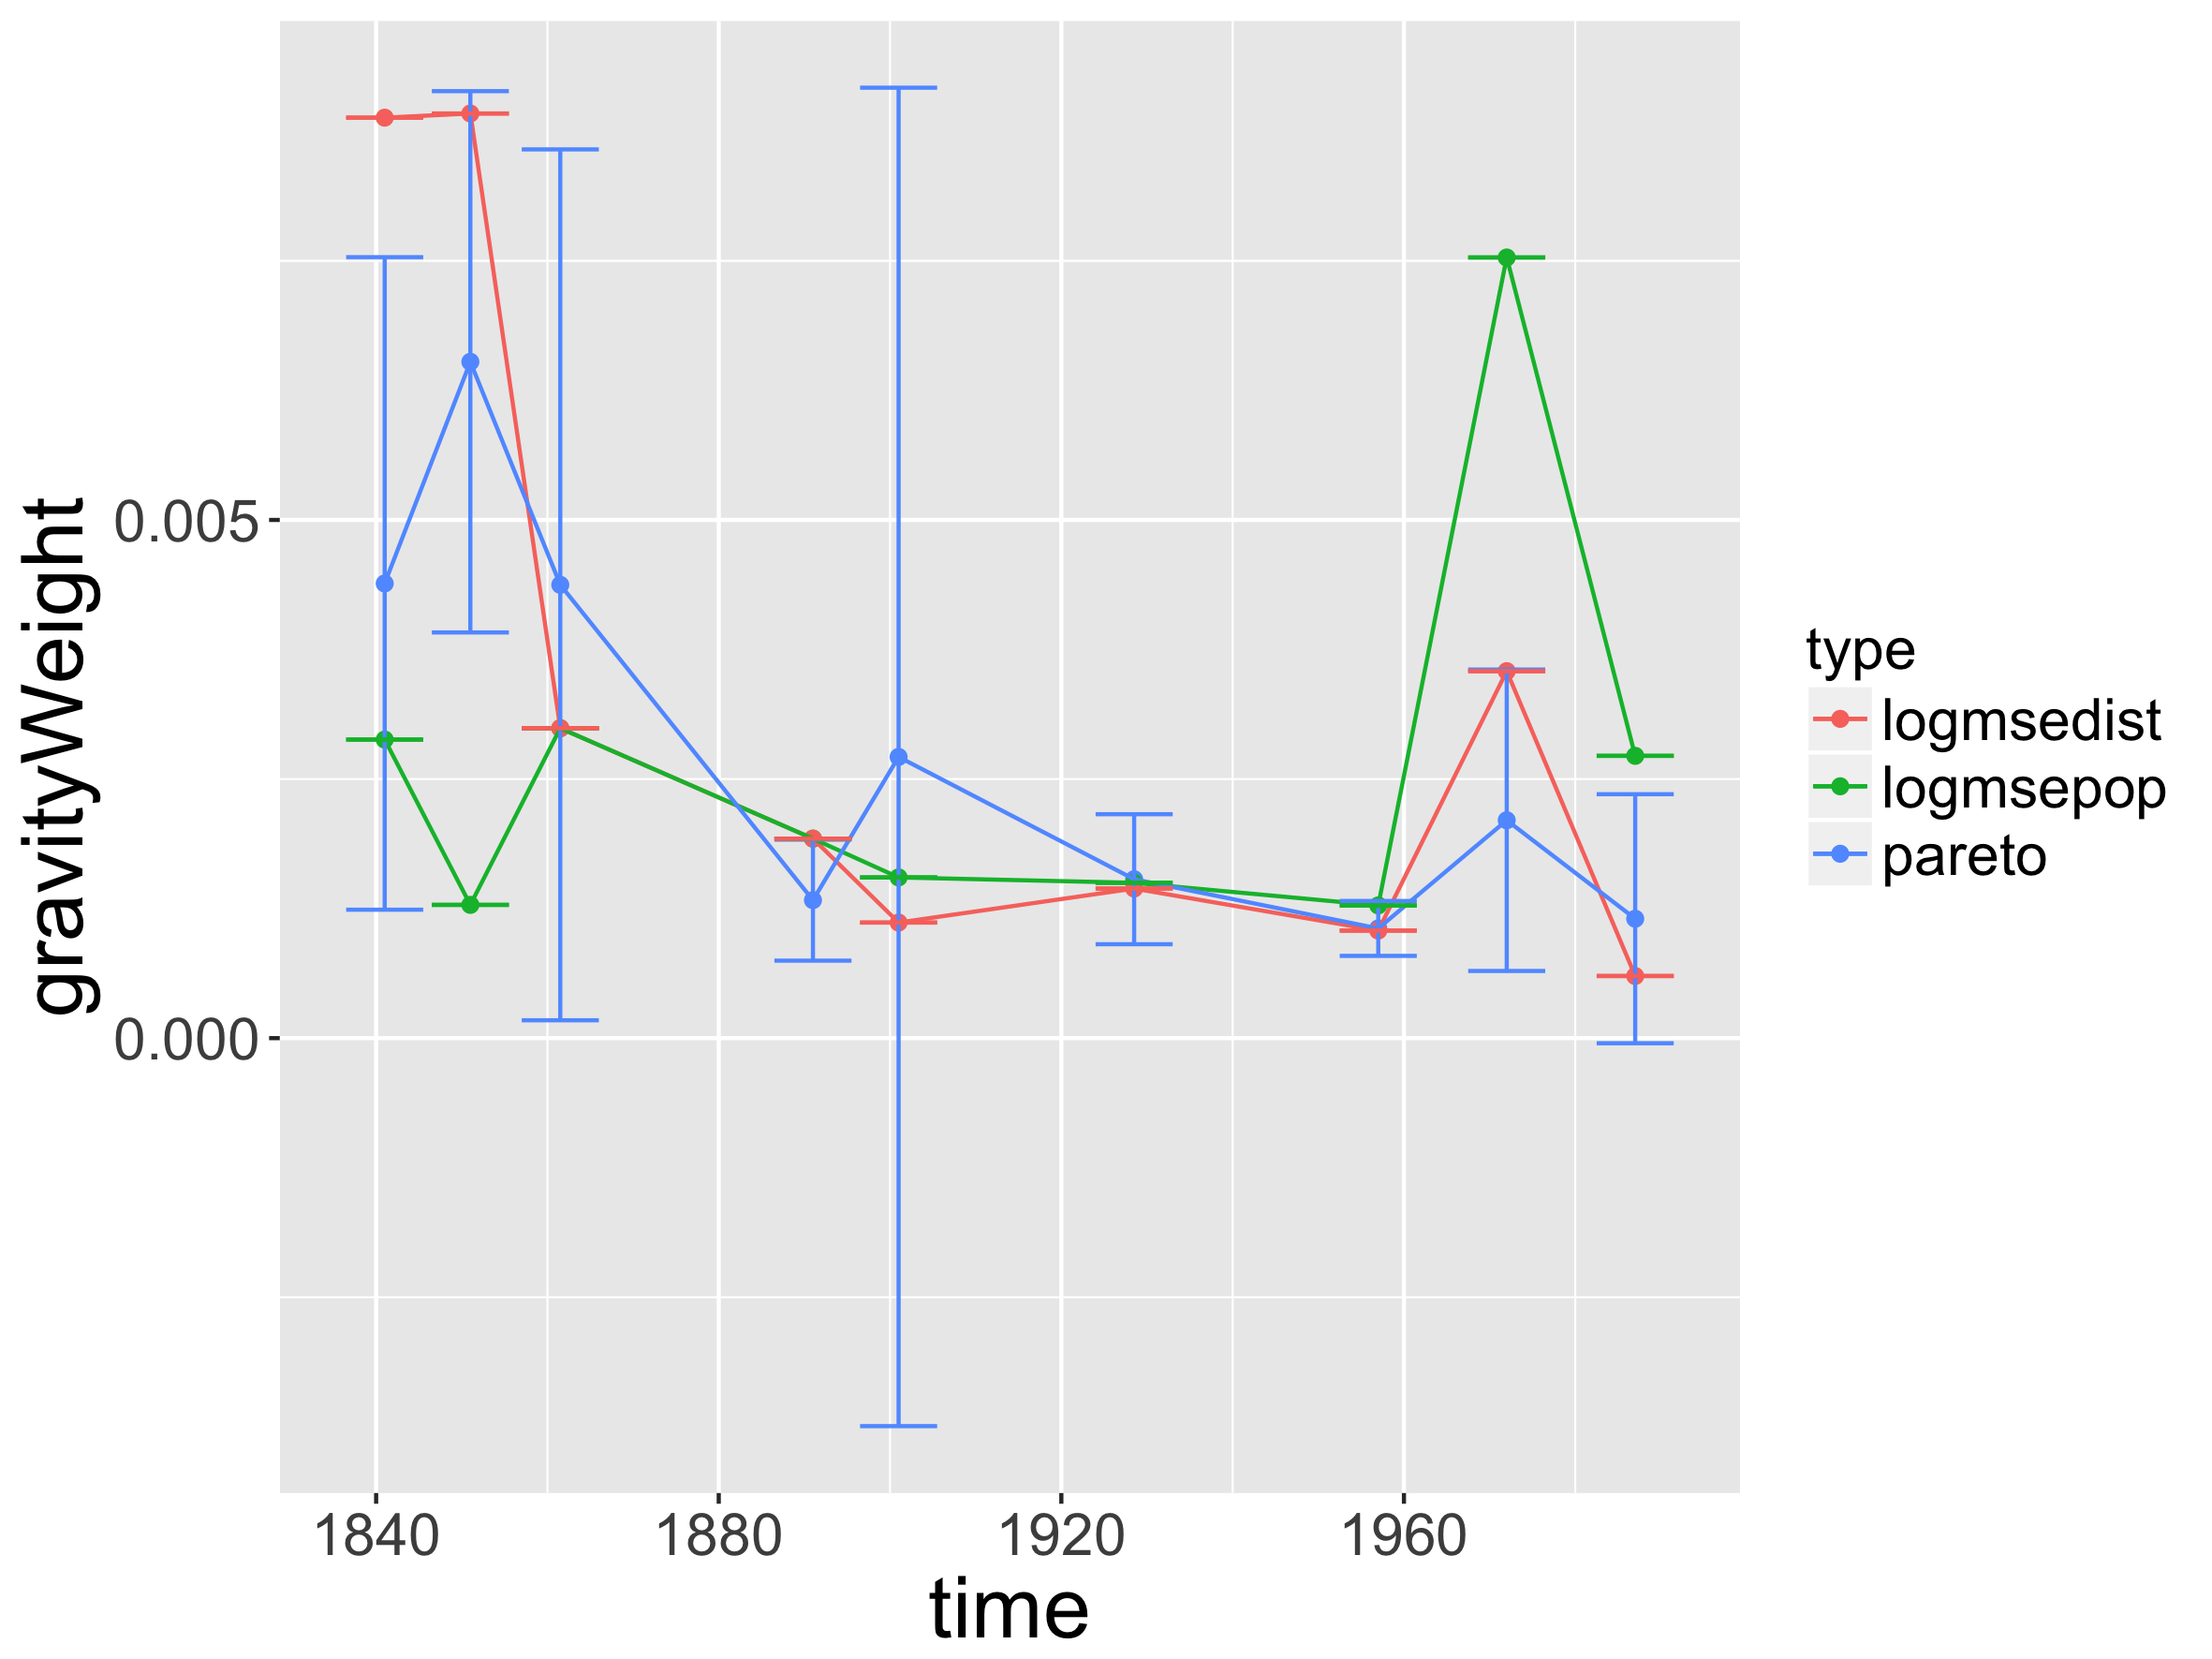
\includegraphics[width=0.32\linewidth]{Figures/MacroCoEvol/param_gravityWeight_filt1}
	%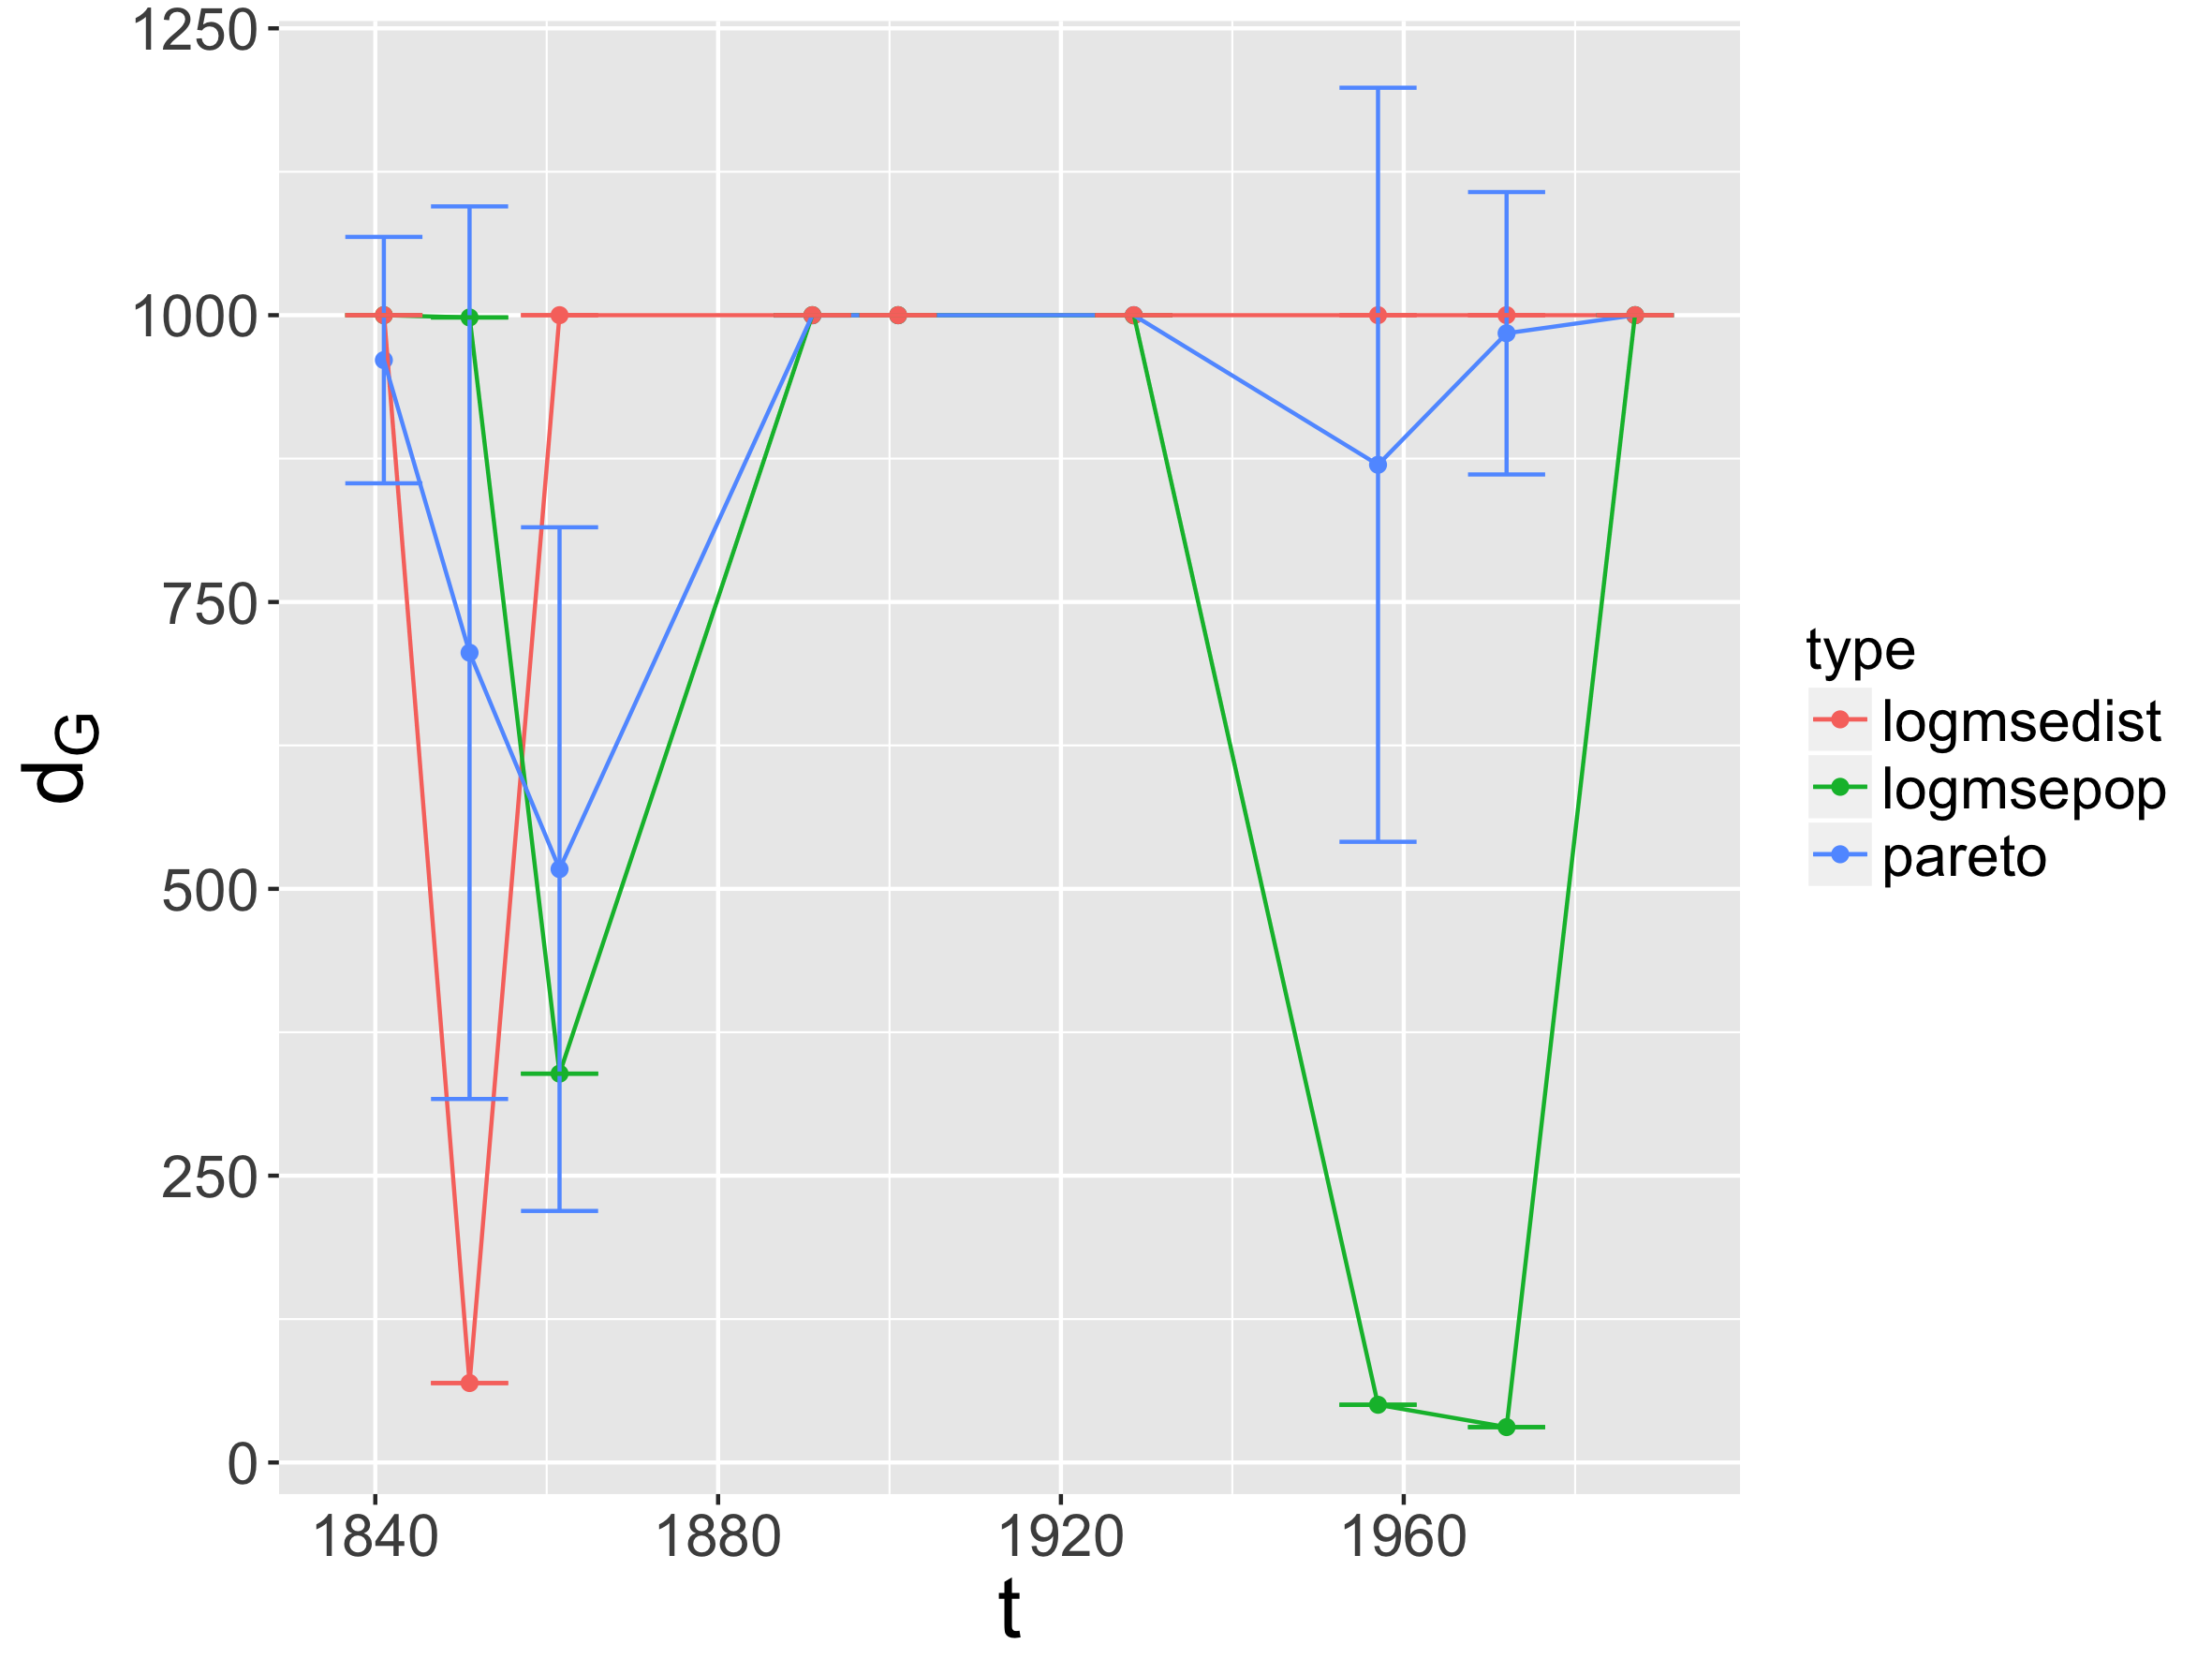
\includegraphics[width=0.32\linewidth]{Figures/MacroCoEvol/param_gravityDecay_filt1}
	%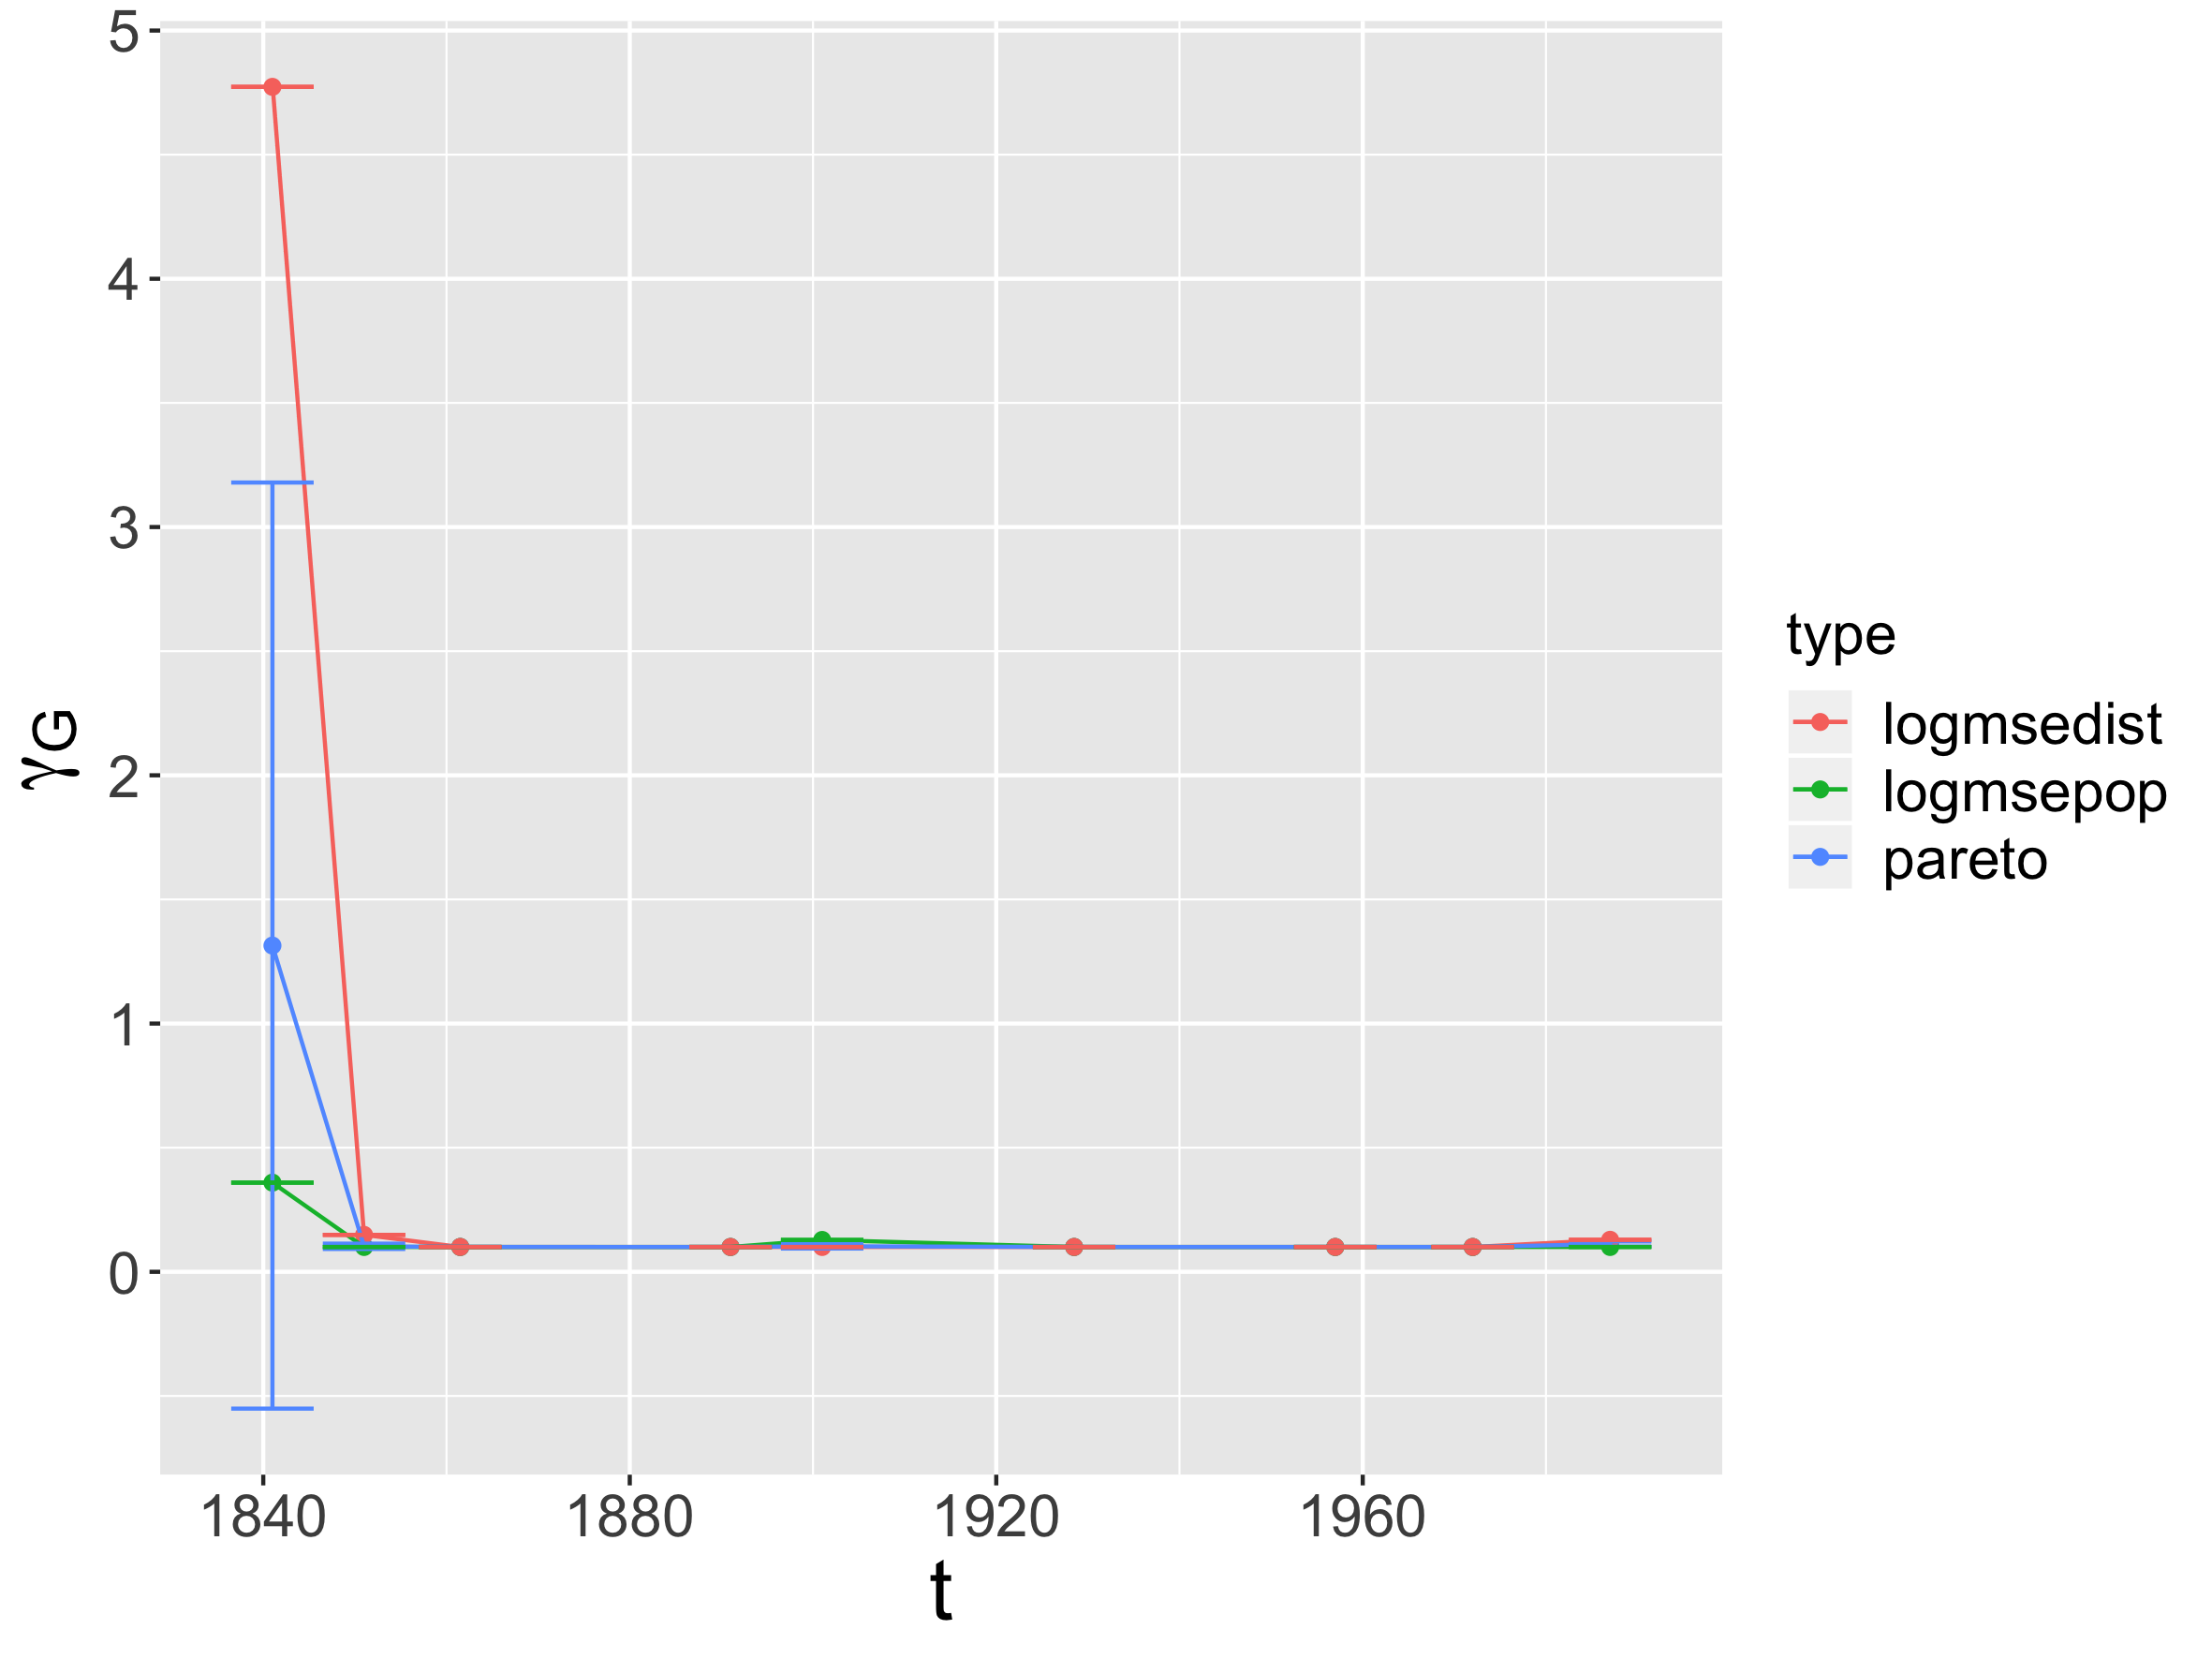
\includegraphics[width=0.32\linewidth]{Figures/MacroCoEvol/param_gravityGamma_filt1}\\
	%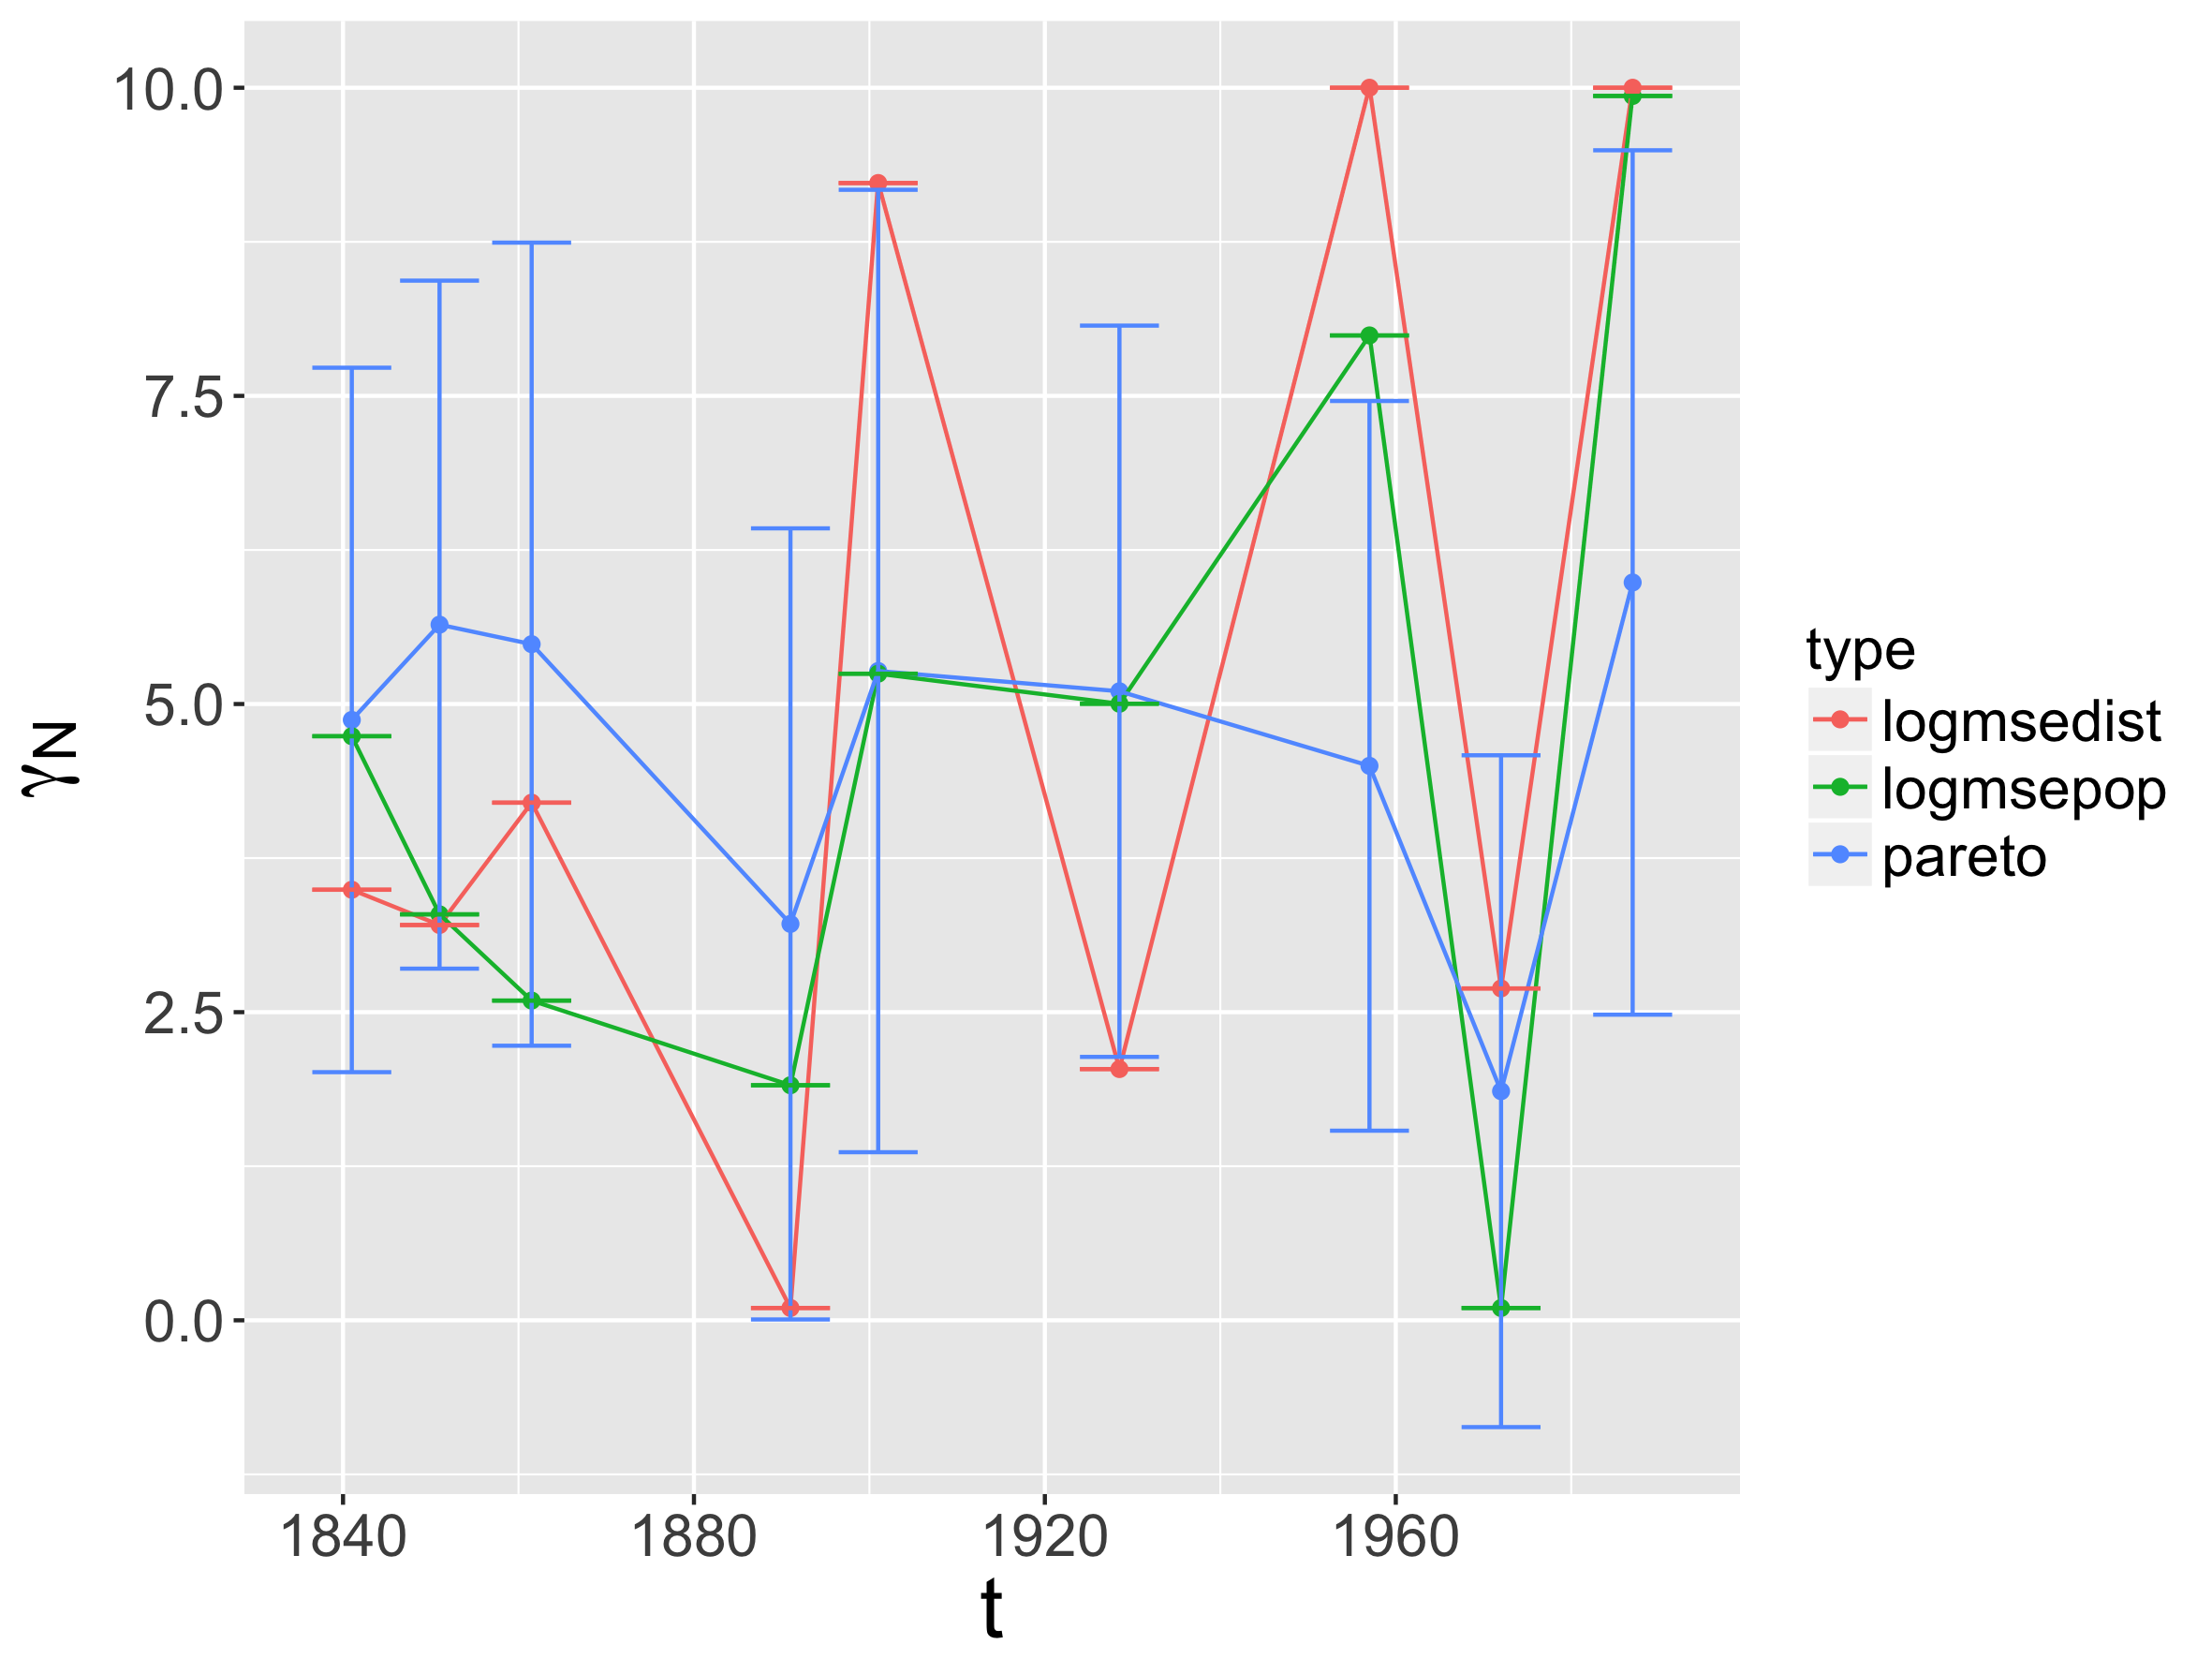
\includegraphics[width=0.32\linewidth]{Figures/MacroCoEvol/param_nwExponent_filt1}
	%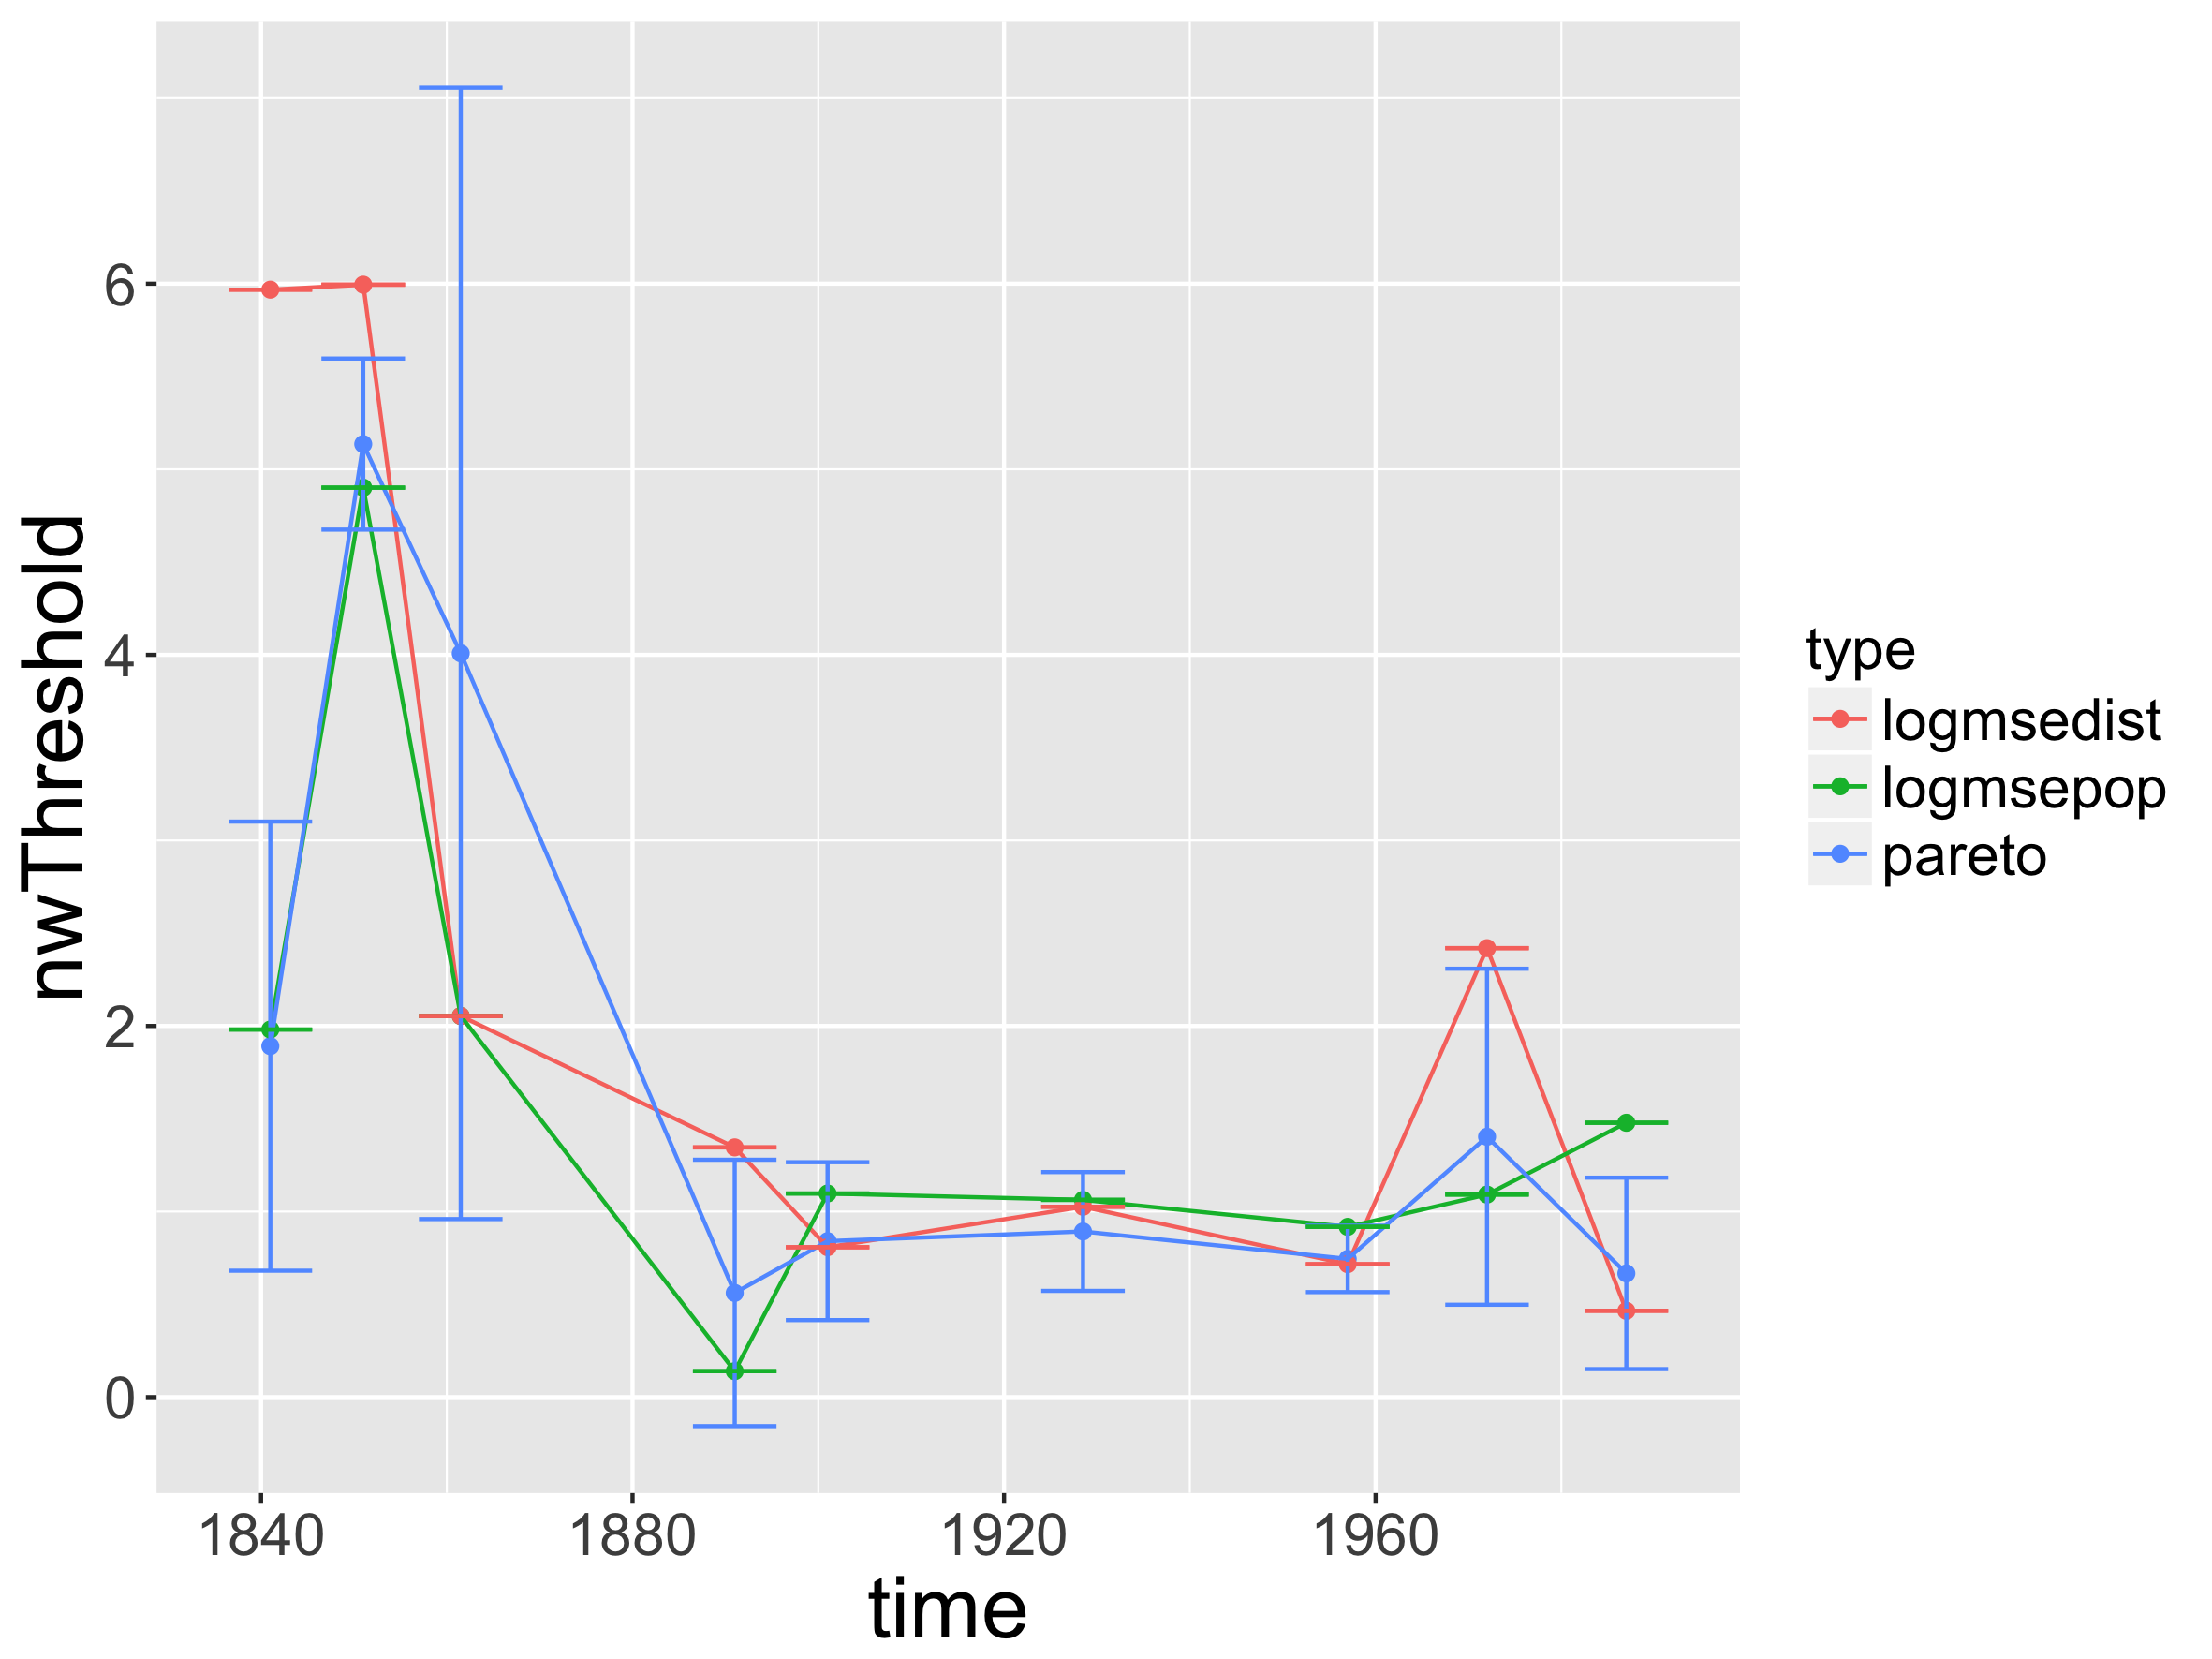
\includegraphics[width=0.32\linewidth]{Figures/MacroCoEvol/param_nwThreshold_filt1}
	%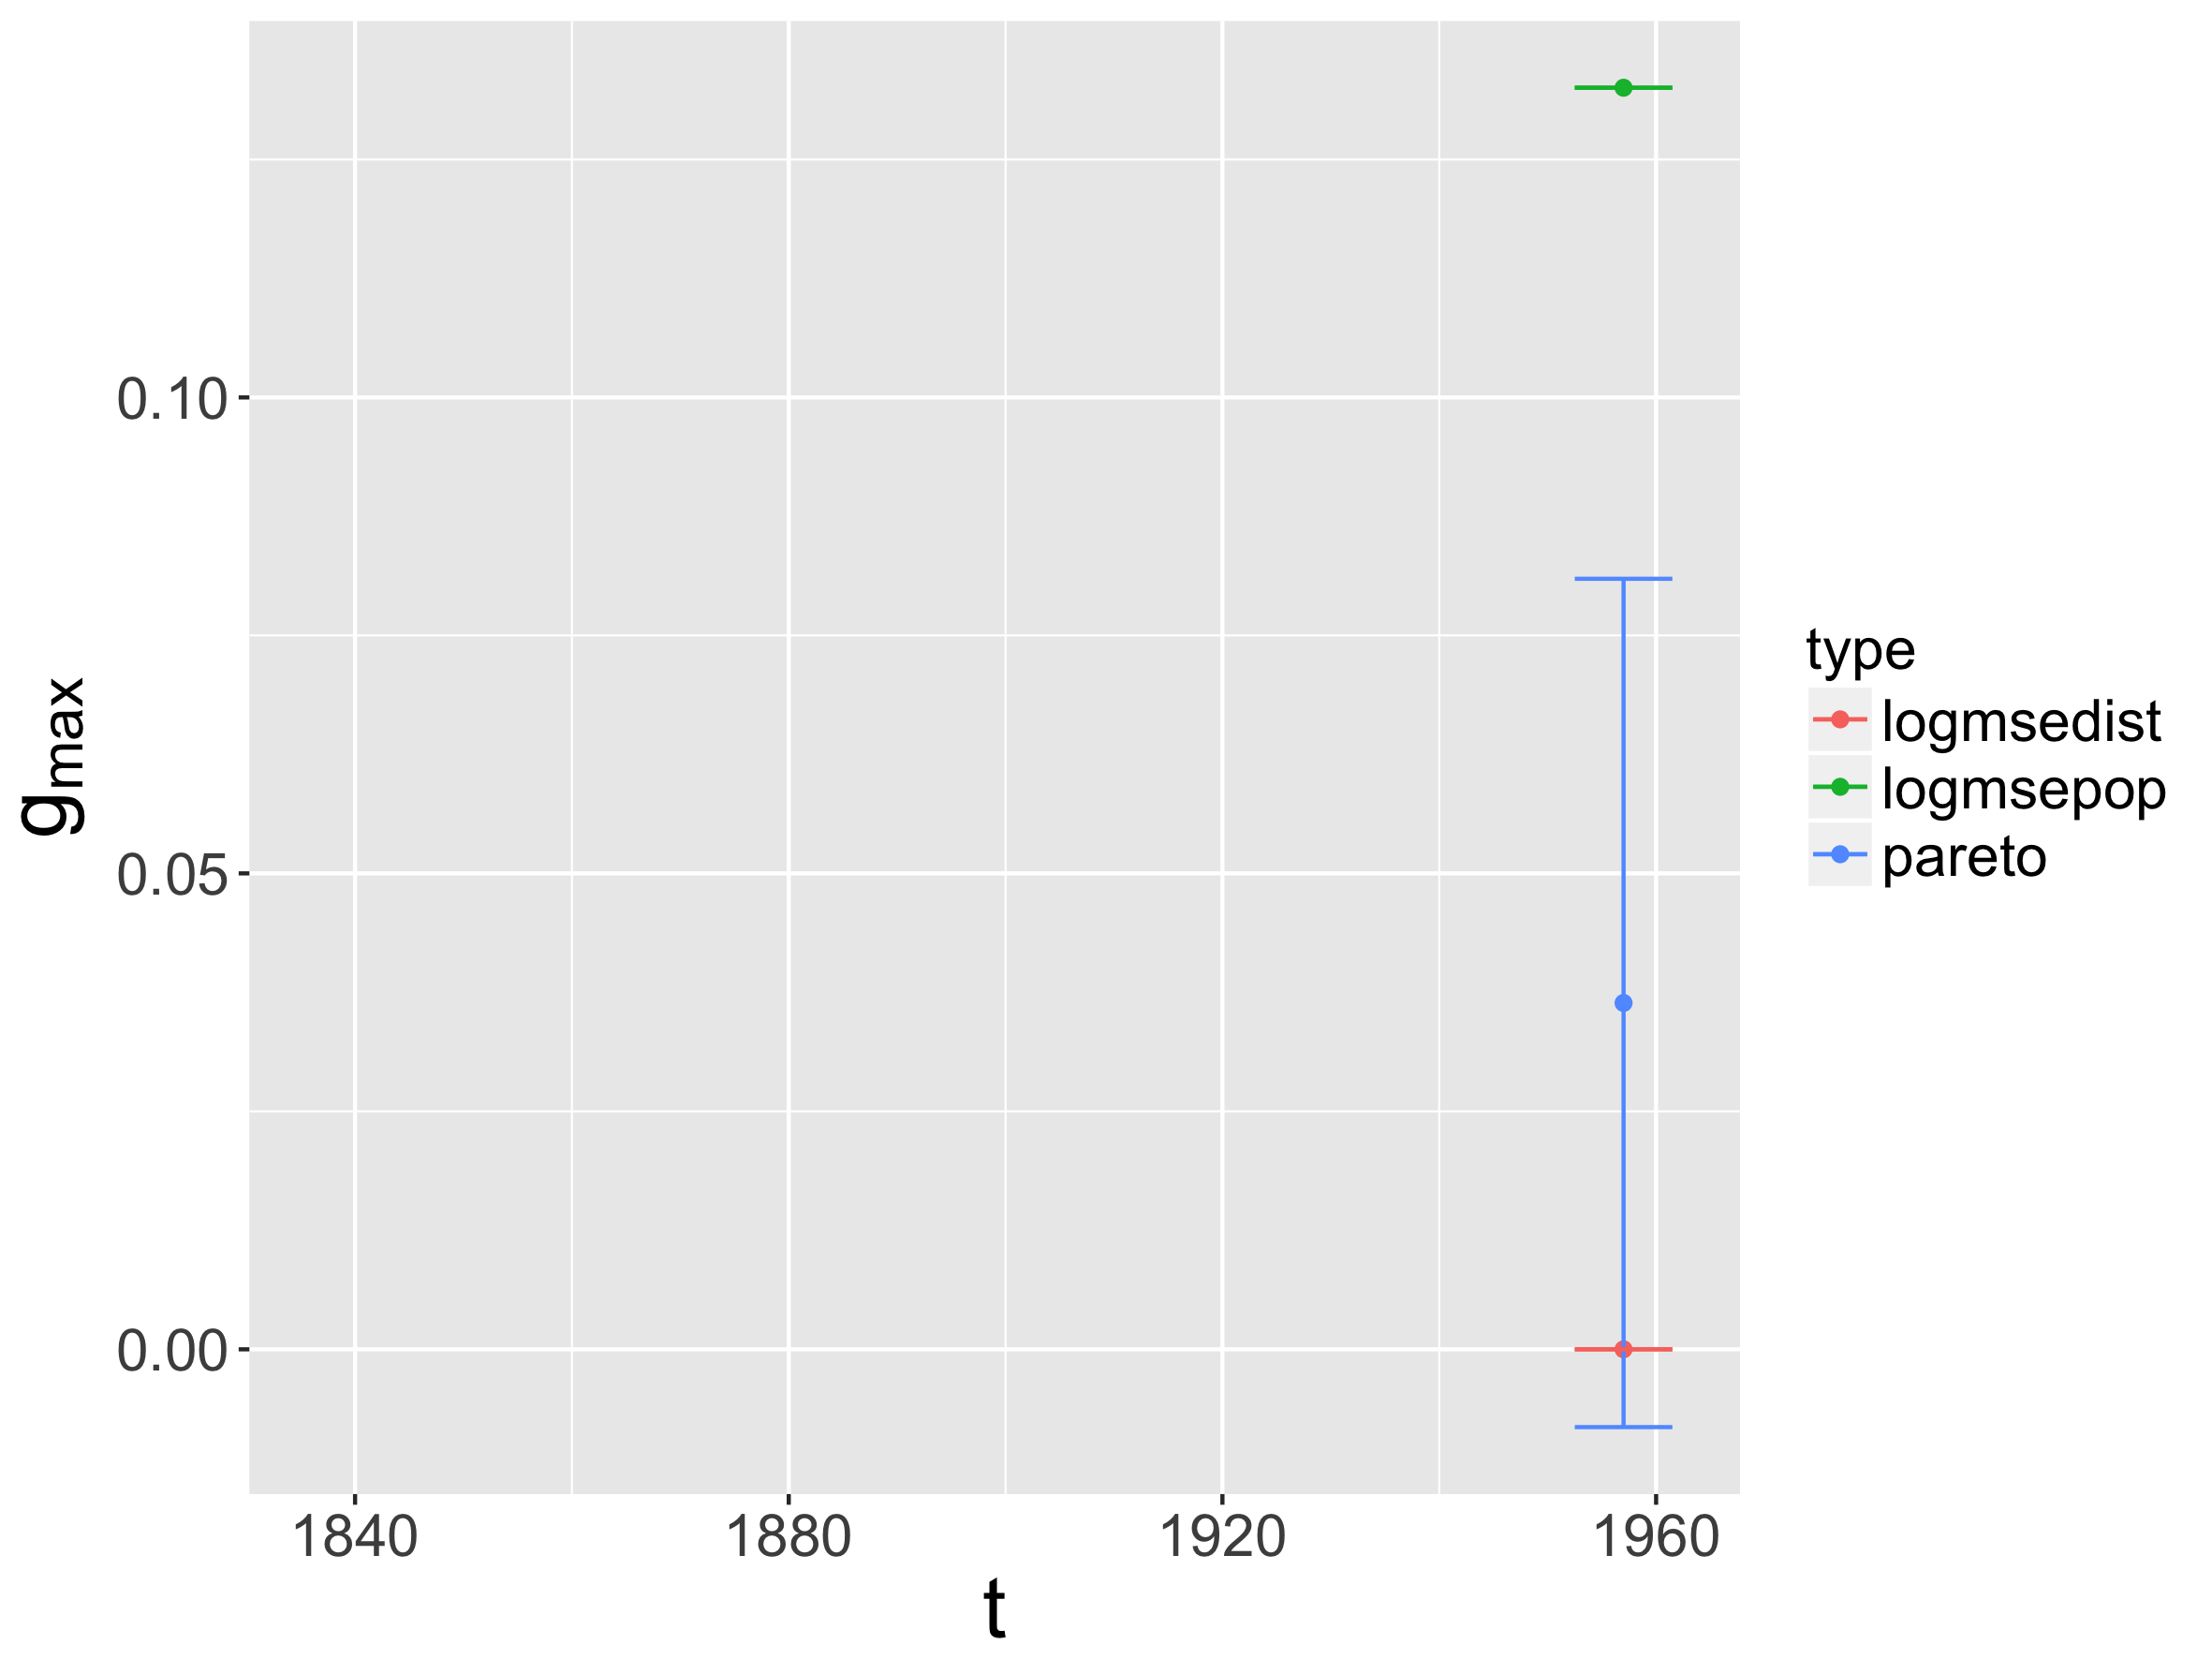
\includegraphics[width=0.32\linewidth]{Figures/MacroCoEvol/param_nwGmax_filt1}
	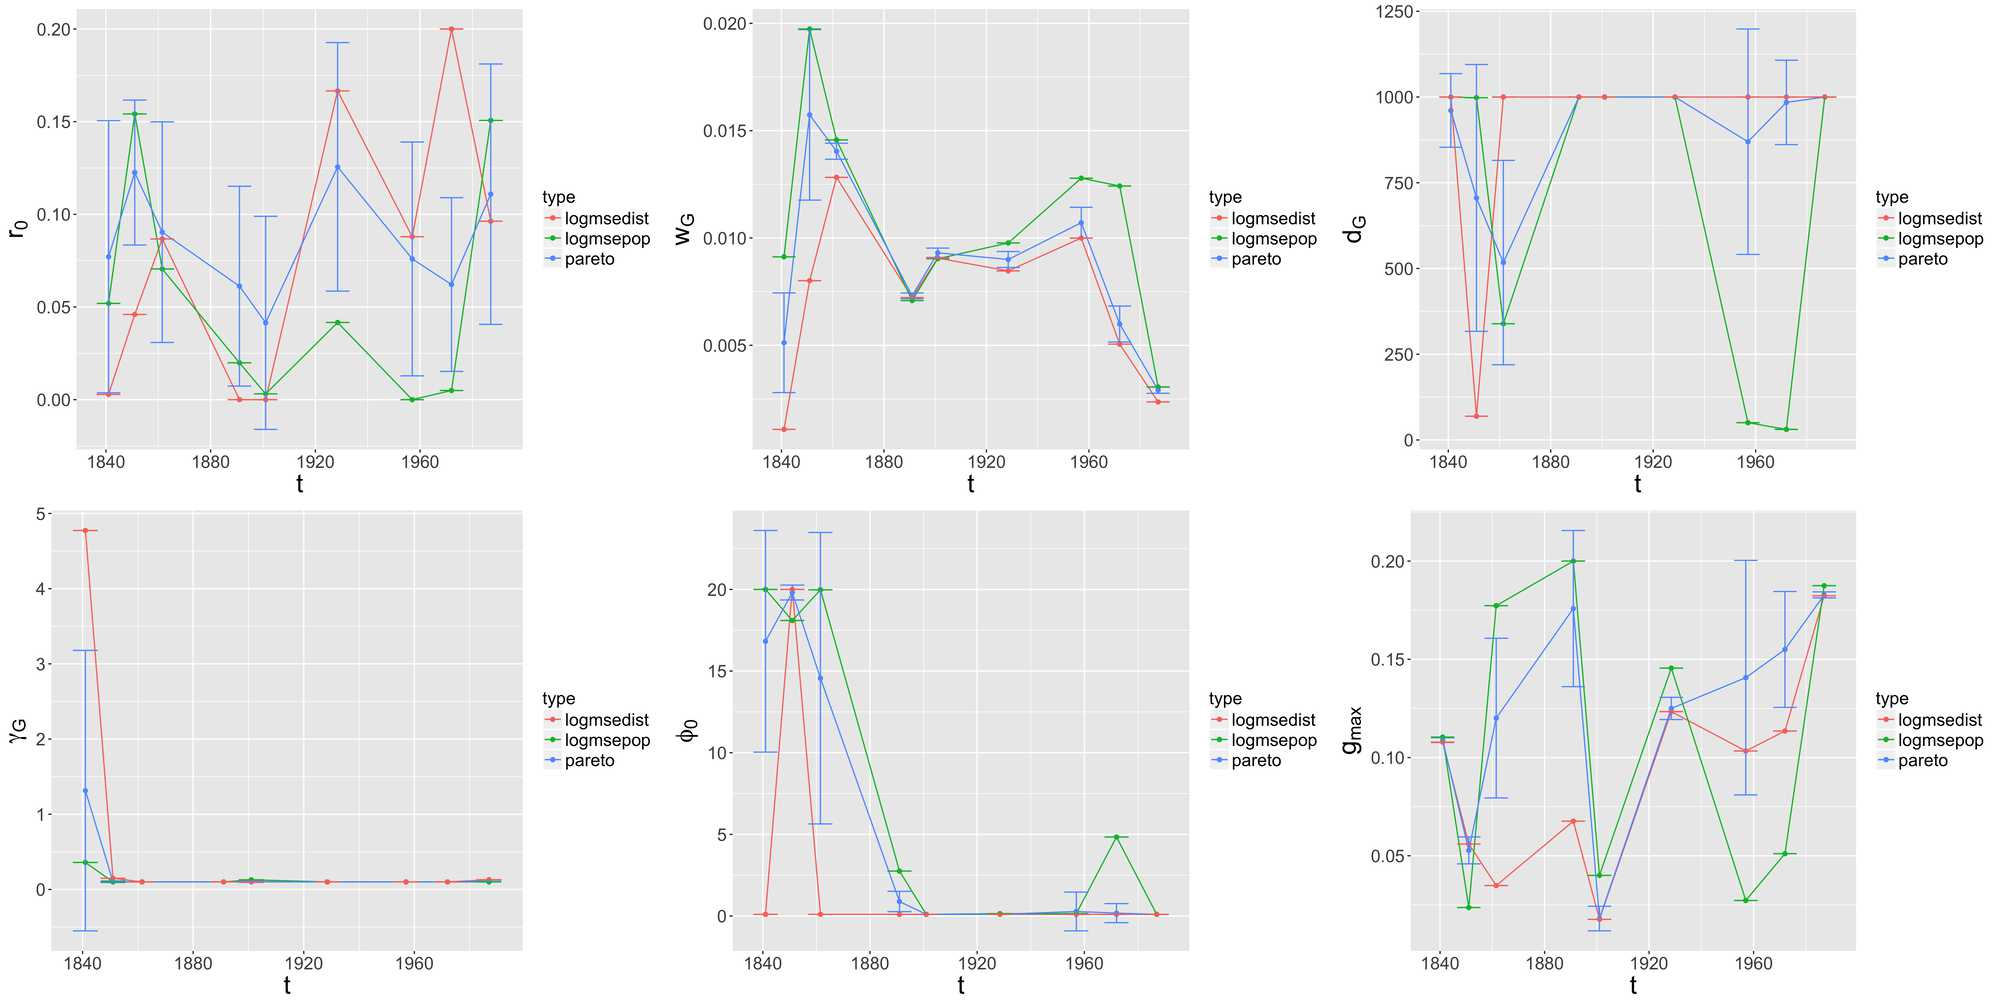
\includegraphics[width=\linewidth]{figures/6-2-3-fig-macrocoevol-parameters.jpg}
	\caption[Evolution of calibrated parameters]{\textbf{Temporal evolution of optimal parameters.} From left to right and top to bottom, values of parameters $(r_0,w_G,d_G,\gamma_G,\phi_0,g_{max})$, respectively for the full Pareto front (blue), for the optimal point in the sense of the distance (red) and the optimal point in the sense of the population (green). \label{fig:macrocoevol:parameters}}
\end{figure}
%%%%%%%%%%%%%%%%%%%


\subsubsection{Model with a physical network}


We now sketch the outline of a specification of the model with a physical network, what would in a sense correspond to an hybrid model combining different scales. The objective of such a specification would be on the one hand to study the difference in trajectories compared to the abstract network, i.e. to quantify the importance of economies of scale (due to common links), of congestion and also the possible compromises to take in order to spatialize the network. On the other hand, it would help to understand to what extent it is possible to produce realistic networks in comparison to autonomous network growth models for example. These issues are tackled at an other scale and for other ontological specifications in chapter~\ref{ch:mesocoevolution}.


Such a specification follows the frame of \cite{li2014modeling}, which model the co-evolution between transportation corridors and the growth of main poles at a regional scale.


The physical network we implement aims at satisfying a greedy criteria of local time gain. More precisely, we assume a self-reinforcement similar to~\cite{tero2010rules} A specification analog to the one used before assumes a growth for each link, given also in a logic of self-reinforcement by:

\[
d(t+1) = d(t)\cdot \left(1 + g_{max} \cdot \left[\frac{\phi}{\max \phi}\right]^{\gamma_s}\right)
\]

if $\phi$ is the flow in the link and $d(t)$ its effective distance. The threshold specification used before does indeed not allow a good convergence in time, in particular with the emergence of local oscillation phenomena.

We generate a random initial network, by perturbing the position of vertices of a grid for which a fixed proportion of links has been removed (40\%) and by linking cities to the network through the shortest path. Links have all the same impedance, which then evolves according to the equation above. An example of a configuration obtained with this specification is given in Fig.~\ref{fig:macrocoevolution:slimemould}. The good convergence properties (visual stabilization of network structure during restricted experiments) suggest the potentialities offered by this specification, which systematic exploration is out of the scope of this work.


%%%%%%%%%%%%%%%%%%%%%%
\begin{figure}
	%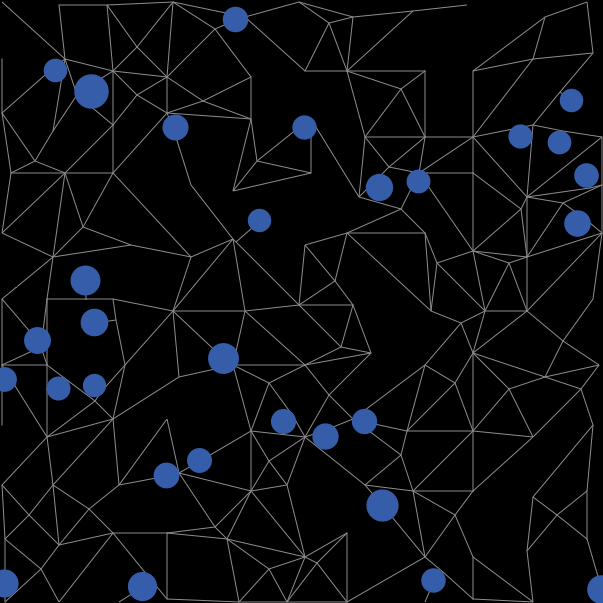
\includegraphics[width=0.45\linewidth]{Figures/MacroCoEvol/example_slimemould_1_t0}
	%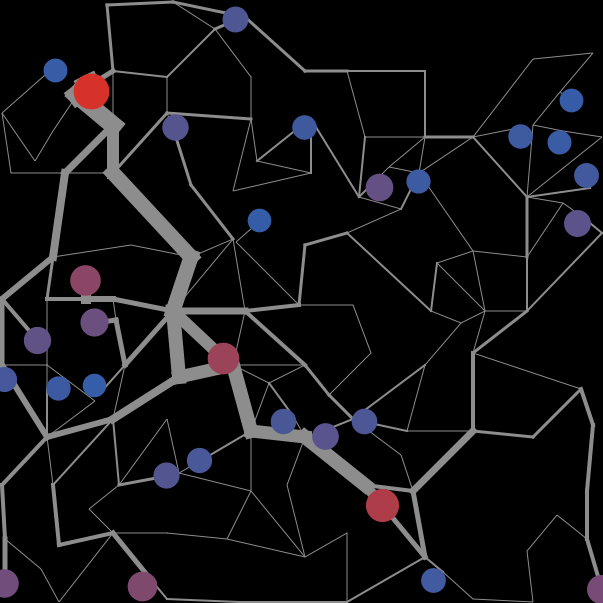
\includegraphics[width=0.45\linewidth]{Figures/MacroCoEvol/example_slimemould_1_tf}
	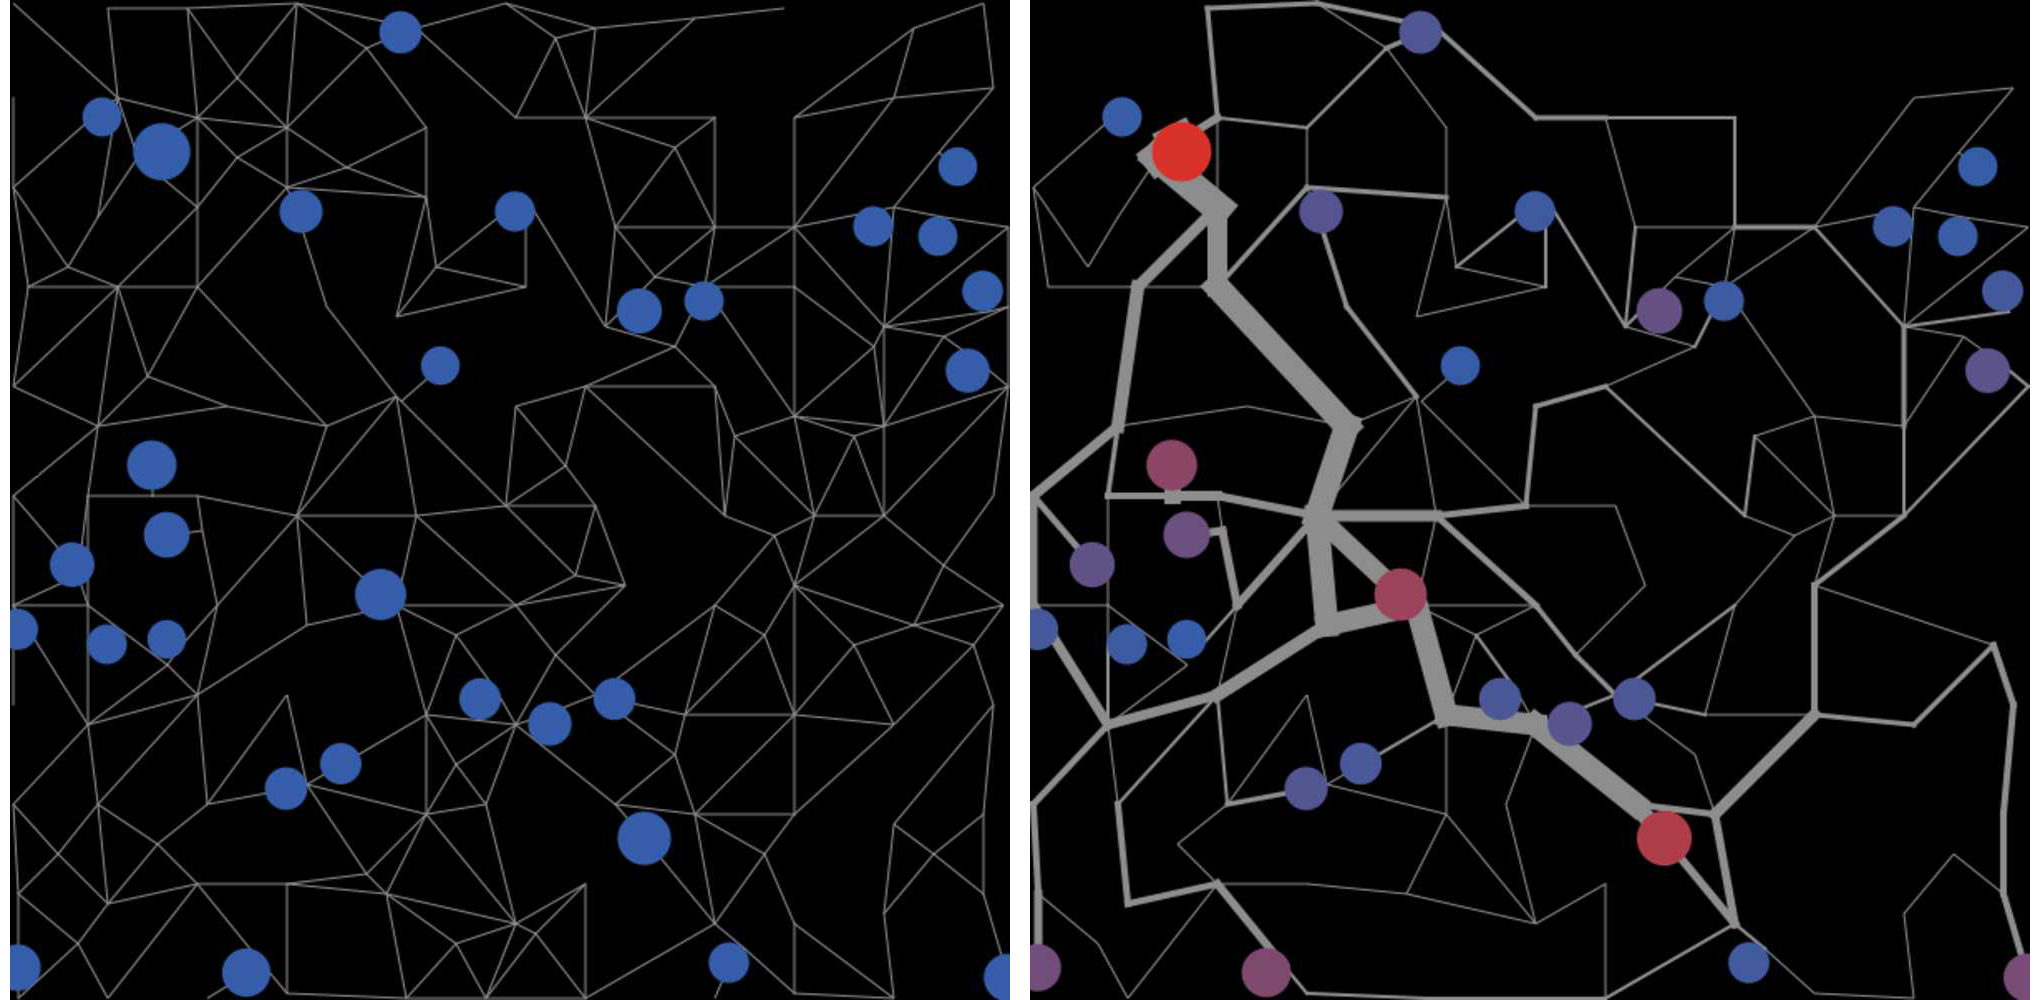
\includegraphics[width=\linewidth]{figures/6-2-3-fig-macrocoevol-slimemould}
	\caption[Example of application of the macroscopic model with a self-reinforcing network]{\textbf{Example of configuration obtained with a self-reinforcing network.} \textit{(Left)} Inital random configuration, with uniform impedances; \textit{(Right)} Final configuration obtained after 100 iterations.\label{fig:macrocoevolution:slimemould}}
\end{figure}
%%%%%%%%%%%%%%%%%%%%%%




\section{Discussion}




\subsection{Application}


The study of particular trajectories within a system of cities can allow to answer to specific thematic questions: for example, the influence of medium-sized cities on the global trajectory of the system, or the drivers of a more or less ``successful'' trajectory for this type of profile. In the case of the application to a real system, the mapping of deviation to the model in time can suggest regional particularities.


\subsection{Developments}


We also finally expect to be able through the model to compare urban systems in different geographical and political contexts, and at different scales. This should foster the understanding the implications of planning actions on the interactions between networks and territories. For example, French railway network has emerged through multiple operators, on the contrary to the Chinese high speed railway network, for which a more precise development could be considered.



\section*{Conclusion}












%%%%%%%%%%%%%%%%%%%%
%% Biblio
%%%%%%%%%%%%%%%%%%%%


%\bibliographystyle{apalike}
%\bibliography{/home/raimbault/ComplexSystems/CityNetwork/Biblio/Bibtex/CityNetwork}

\begin{thebibliography}{}

\bibitem[Berroir et~al., 2017]{berroir2017systemes}
Berroir, S., Cattan, N., Dobruszkes, F., Gu{\'e}rois, M., Paulus, F., and
  Vacchiani-Marcuzzo, C. (2017).
\newblock Les syst{\`e}mes urbains fran{\c{c}}ais: une approche relationnelle.
\newblock {\em Cybergeo: European Journal of Geography}.

\bibitem[Bretagnolle, 2003]{bretagnolle2003vitesse}
Bretagnolle, A. (2003).
\newblock Vitesse et processus de s{\'e}lection hi{\'e}rarchique dans le
  syst{\`e}me des villes fran{\c{c}}aises.
\newblock {\em Donn{\'e}es urbaines}, 4.

\bibitem[Cottineau, 2017]{10.1371/journal.pone.0183919}
Cottineau, C. (2017).
\newblock Metazipf. a dynamic meta-analysis of city size distributions.
\newblock {\em PLOS ONE}, 12(8):1--22.

\bibitem[Gu{\'e}rois and Pumain, 2008]{guerois2008built}
Gu{\'e}rois, M. and Pumain, D. (2008).
\newblock Built-up encroachment and the urban field: a comparison of forty
  european cities.
\newblock {\em Environment and Planning A}, 40(9):2186--2203.

\bibitem[Holland, 2012]{holland2012signals}
Holland, J.~H. (2012).
\newblock {\em Signals and boundaries: Building blocks for complex adaptive
  systems}.
\newblock MIT Press.

\bibitem[Jacobs-Crisioni and Koopmans, 2016]{jacobs2016transport}
Jacobs-Crisioni, C. and Koopmans, C.~C. (2016).
\newblock Transport link scanner: simulating geographic transport network
  expansion through individual investments.
\newblock {\em Journal of Geographical Systems}, 18(3):265--301.

\bibitem[Lemoy and Caruso, 2017]{lemoy2017scaling}
Lemoy, R. and Caruso, G. (2017).
\newblock Scaling evidence of the homothetic nature of cities.
\newblock {\em arXiv preprint arXiv:1704.06508}.

\bibitem[Levinson and Xie, 2011]{levinson2011does}
Levinson, D. and Xie, F. (2011).
\newblock Does first last? the existence and extent of first mover advantages
  on spatial networks.
\newblock {\em Journal of Transport and Land Use}.

\bibitem[Li et~al., 2014]{li2014modeling}
Li, Y., Lu, D., and Tian, Y. (2014).
\newblock Modeling corridor and growth pole coevolution in regional
  transportation network.
\newblock {\em Transportation Research Record: Journal of the Transportation
  Research Board}, (2466):144--152.

\bibitem[Mimeur et~al., 2017]{mimeur:hal-01616746}
Mimeur, C., Queyroi, F., Banos, A., and Th{\'e}venin, T. (2017).
\newblock {Revisiting the structuring effect of transportation infrastructure:
  an empirical approach with the French Railway Network from 1860 to 1910}.
\newblock {\em {Historical Methods: A Journal of Quantitative and
  Interdisciplinary History}}.

\bibitem[Offner et~al., 2014]{espacegeo2014effets}
Offner, J.-M., Beaucire, F., Delaplace, M., Fr{\'e}mont, A., Ninot, O.,
  Bretagnolle, A., and Pumain, D. (2014).
\newblock Les effets structurants des infrastructures de transport.
\newblock {\em Espace Geographique}, (42):p--51.

\bibitem[Tero et~al., 2007]{tero2007mathematical}
Tero, A., Kobayashi, R., and Nakagaki, T. (2007).
\newblock A mathematical model for adaptive transport network in path finding
  by true slime mold.
\newblock {\em Journal of theoretical biology}, 244(4):553--564.

\bibitem[Tero et~al., 2010]{tero2010rules}
Tero, A., Takagi, S., Saigusa, T., Ito, K., Bebber, D.~P., Fricker, M.~D.,
  Yumiki, K., Kobayashi, R., and Nakagaki, T. (2010).
\newblock Rules for biologically inspired adaptive network design.
\newblock {\em Science}, 327(5964):439--442.

\bibitem[Th{\'e}venin et~al., 2013]{thevenin2013mapping}
Th{\'e}venin, T., Schwartz, R., and Sapet, L. (2013).
\newblock Mapping the distortions in time and space: The french railway network
  1830--1930.
\newblock {\em Historical Methods: A Journal of Quantitative and
  Interdisciplinary History}, 46(3):134--143.

\bibitem[Zembri, 1997]{zembri1997fondements}
Zembri, P. (1997).
\newblock Les fondements de la remise en cause du sch{\'e}ma directeur des
  liaisons ferroviaires {\`a} grande vitesse: des faiblesses avant tout
  structurelles.
\newblock In {\em Annales de g{\'e}ographie}, pages 183--194. JSTOR.

\end{thebibliography}




\end{document}
